\documentclass[11pt,a4paper]{article}
\usepackage[utf8]{inputenc}
\usepackage[T1]{fontenc}
\usepackage[spanish,es-noindentfirst,es-tabla]{babel}
\usepackage{lmodern}
\usepackage{amsmath,amssymb}
\usepackage{booktabs}
\usepackage{tabularx}
\usepackage{graphicx}
\usepackage{listings}
\usepackage{xcolor}
\usepackage[hidelinks]{hyperref}
\usepackage{cite}
\usepackage{float}
\usepackage{geometry}
\geometry{a4paper, margin=2.0cm, headheight=14pt}
\usepackage{array}
\usepackage{enumitem}
\usepackage{caption}
\usepackage{fancyhdr}
\usepackage{microtype}
\usepackage{multirow}

\pagestyle{fancy}
\fancyhf{}
\fancyhead[L]{\small\color{gray} UTEQ -- Aplicaciones Distribuidas [ISR-701]}
\fancyhead[R]{\small\color{gray} AcadTrace: PFC E4 -- Sistema de Gestión Académica Distribuido}
\fancyfoot[C]{\thepage}
\renewcommand{\headrulewidth}{0.4pt}
\renewcommand{\footrulewidth}{0.4pt}

\definecolor{codegreen}{rgb}{0.15,0.55,0.15}
\definecolor{codegray}{rgb}{0.45,0.45,0.45}
\definecolor{backcolour}{rgb}{0.97,0.98,0.99}
\definecolor{codeblue}{rgb}{0.1,0.25,0.7}
\definecolor{codered}{rgb}{0.75,0.1,0.1}

\lstdefinelanguage{json}{
  basicstyle=\ttfamily\scriptsize,
  showstringspaces=false,
  breaklines=true,
  stringstyle=\color{codered},
  keywordstyle=\color{codeblue}\bfseries,
  commentstyle=\color{codegreen}\itshape,
  morestring=[b]",
  morestring=[d]'
}

\lstdefinelanguage{yaml}{
  keywords={name,on,push,pull_request,branches,env,jobs,steps,uses,with,run,needs,if,runs-on},
  keywordstyle=\color{codeblue}\bfseries,
  basicstyle=\ttfamily\scriptsize,
  sensitive=false,
  comment=[l]{\#},
  commentstyle=\color{codegreen}\itshape,
  stringstyle=\color{codered},
  morestring=[b]',
  morestring=[b]"
}

\lstdefinestyle{codigo}{
  backgroundcolor=\color{backcolour},
  commentstyle=\color{codegreen}\itshape,
  keywordstyle=\color{codeblue}\bfseries,
  numberstyle=\tiny\color{codegray},
  stringstyle=\color{codered},
  basicstyle=\ttfamily\scriptsize,
  breakatwhitespace=false,
  breaklines=true,
  captionpos=b,
  keepspaces=true,
  numbers=left,
  numbersep=5pt,
  showspaces=false,
  showstringspaces=false,
  showtabs=false,
  tabsize=2,
  frame=single,
  rulecolor=\color{codegray!30}
}
\lstset{style=codigo}

% Generado desde el conjunto A por scripts/recalcular_metricas_carga.py
\newcommand{\CargaPeticiones}{12994}
\newcommand{\CargaFallos}{0}
\newcommand{\CargaRPS}{43.53758011606015}
\newcommand{\CargaMediaMs}{109.1136640344576}
\newcommand{\CargaPcinquentaMs}{6}
\newcommand{\CargaPnoventaCincoMs}{440}
\newcommand{\CargaPnoventaNueveMs}{850}
\newcommand{\CargaUsuariosMaximos}{50}


\begin{document}

% =============================================================================
% PORTADA INSTITUCIONAL OFICIAL (CRITERIO PISO P1: URL EN UNA LÍNEA)
% =============================================================================
\begin{titlepage}
\centering
\vspace*{0.2cm}

\includegraphics[width=0.25\textwidth]{FCClogo.jpg}\par
\vspace{0.3cm}
{\Large\bfseries UNIVERSIDAD T\'ECNICA ESTATAL DE QUEVEDO\par}
\vspace{0.15cm}
{\large\bfseries FACULTAD DE CIENCIAS DE LA COMPUTACI\'ON\par}
{\large CARRERA DE INGENIER\'IA DE SOFTWARE\par}
\vspace{0.6cm}
\rule{\textwidth}{1.2pt}\\[0.3cm]
{\Large\bfseries PROYECTO FIN DE CURSO (PFC) -- INFORME INTEGRAL ENTREGA 4\par}
\vspace{0.2cm}
{\large\bfseries AcadTrace: Capa de Auditor\'ia Criptogr\'afica Verificable y Gesti\'on Acad\'emica Distribuida con Protocolos H\'ibridos gRPC/REST, Observabilidad Multi-Nivel y Pipeline CI/CD Automatizado\par}
\rule{\textwidth}{1.2pt}\\[0.5cm]

\textbf{Asignatura:} Aplicaciones Distribuidas (ISR-701) -- S\'eptimo Semestre\\[0.1cm]
\textbf{Per\'iodo Acad\'emico:} Regular 2026--2027\\[0.1cm]
\textbf{Equipo de Trabajo:} BCEL (Escuela Provincias Unidas)\\[0.4cm]

\begin{tabular}{ll}
\textbf{Castro L\'opez Pedro Leonardo} & Arquitecto de Software y L\'ider de Proyecto \\
\textbf{Bedon Viteri Keyla Betzabe} & Responsable de Microservicio Docente y App M\'ovil \\
\textbf{Luna Mora Ernesto Gregory} & Responsable de Microservicio Secretar\'ia y Calidad \\
\textbf{Emanuel Pino Juliana Romina} & Responsable de Microservicio Soporte y Observabilidad \\
\end{tabular}

\vspace{0.5cm}
\textbf{Docente Revisor:}\\[0.1cm]
Prof. Ing. Gleiston C. Guerrero-Ulloa, Mgs.

\vspace{0.5cm}
\textbf{Repositorio Oficial de C\'odigo y Evidencias Reproducibles (Criterio Piso P1):}\\[0.1cm]
\url{https://github.com/LEO23as/acadtrace}

\vspace{0.4cm}
{\small Quevedo, Los R\'ios, Ecuador -- Septiembre 2026\par}
\end{titlepage}

\pagenumbering{roman}
\tableofcontents
\newpage
\pagenumbering{arabic}

% =============================================================================
% RESUMEN BILINGÜE
% =============================================================================
\section*{Resumen y Abstract}
\addcontentsline{toc}{section}{Resumen y Abstract}

\noindent\textbf{Resumen}---El presente trabajo expone el dise\~no, refactorizaci\'on, despliegue y evaluaci\'on experimental de \textbf{AcadTrace}, un sistema de gesti\'on acad\'emica distribuido dotado de una capa de auditor\'ia criptogr\'afica inmutable sobre PostgreSQL con separaci\'on l\'ogica multiesquema. Frente a las limitaciones de trazabilidad en sistemas educativos tradicionales, se implement\'o una arquitectura pol\'iglota de cuatro microservicios (Java Spring Boot, Python Django REST, Node.js Express) interconectados mediante protocolos h\'ibridos (gRPC con HTTP/2 interno y REST perimetral bajo HAProxy). Se integraron cinco patrones de dise\~no GoF, desacoplando el dominio de la infraestructura. La soluci\'on incorpora dos aplicaciones cliente: un portal Web SPA con control de acceso por roles e internacionalizaci\'on, y un cliente m\'ovil nativo Android concebido para representantes de alumnos, con sincronizaci\'on \textit{offline-first}, soporte biom\'etrico y notificaciones push. La evaluaci\'on experimental seg\'un ISO/IEC 25010 mediante 600 corridas factoriales demostr\'o una tasa de detecci\'on del 100\% en los cinco tipos de manipulaci\'on T1--T5 bajo los mecanismos protegidos m2 y m3, basados en encadenamiento SHA-256 y metadatos de orden l\'ogico, con latencia cuantificada únicamente mediante un microbenchmark local secuencial en memoria. La corrida nominal local actual de Soporte conserva \CargaPeticiones{} peticiones con \CargaFallos{} fallos; las corridas históricas fallidas no permiten certificar estrés exitoso ni atribuir por sí solas la causa raíz al pool de conexiones. El ciclo de vida est\'a soportado por un pipeline CI/CD de siete trabajos encadenados y un panel de observabilidad en Grafana de seis vistas en tiempo real.\par

\vspace{0.4cm}
\noindent\textbf{Abstract}---This work presents the design, refactoring, deployment, and experimental evaluation of \textbf{AcadTrace}, a distributed academic management system equipped with an immutable cryptographic audit layer over PostgreSQL with logical schema separation. Addressing the traceability shortcomings of traditional educational software, a polyglot microservice architecture was developed across four services (Java Spring Boot, Python Django REST, Node.js Express), interconnected via hybrid protocols (internal gRPC over HTTP/2 and perimeter REST via HAProxy). Five GoF design patterns were applied to isolate domain logic from infrastructure details. The solution includes two client applications: a responsive Web SPA featuring role-based access control and internationalization, and a native Android mobile client tailored for student guardians, incorporating offline-first synchronization, biometric authentication, and push notifications. Experimental evaluation under ISO/IEC 25010 through 600 factorial runs verified a 100\% detection rate across the five T1--T5 tampering types under the protected m2 and m3 mechanisms, based on SHA-256 hash chaining and logical-order metadata, with latency quantified only through a local sequential in-memory microbenchmark. The official local nominal Support run preserves \CargaPeticiones{} requests with \CargaFallos{} failures. Historical failed runs do not certify successful stress testing or independently establish connection pool exhaustion as their root cause. The operational lifecycle is governed by an end-to-end seven-job CI/CD pipeline and a six-view real-time Grafana observability dashboard.\par

\vspace{0.3cm}
\noindent\textbf{Palabras Clave:} Sistemas Distribuidos, Auditor\'ia Criptogr\'afica, Relojes L\'ogicos de Lamport, Relojes Vectoriales, gRPC, Microservicios, ISO/IEC 25010, CI/CD, Observabilidad.

\newpage

% =============================================================================
% 1. INTRODUCCIÓN Y CONTEXTO
% =============================================================================
\section{Introducci\'on y Contextualizaci\'on del Problema}
\label{sec:introduccion}
La gesti\'on acad\'emica en instituciones educativas de educaci\'on b\'asica demanda soluciones tecnol\'ogicas que garanticen alta disponibilidad, integridad estricta de expedientes escolares, escalabilidad ante picos de matr\'icula y una observabilidad profunda del estado operacional~\cite{newman2021microservices,burns2025designing}. El SGA Escuela Provincias Unidas evolucion\'o desde una arquitectura monol\'itica preliminar hacia una arquitectura distribuida orientada a microservicios desacoplados.

Los esquemas convencionales de persistencia centralizada y bit\'acoras de auditor\'ia pasivas almacenadas en texto plano presentan tres vulnerabilidades estructurales cr\'iticas:
\begin{enumerate}[leftmargin=*]
  \item \textbf{Vulnerabilidad a manipulaciones no autorizadas en base de datos:} Un operador con privilegios de administraci\'on puede alterar directamente los registros en las tablas (\textit{Direct DB Tampering}) sin dejar rastro verificable en la aplicaci\'on.
  \item \textbf{P\'erdida del orden causal en modificaciones concurrentes:} Cuando m\'ultiples docentes o directivos actualizan calificaciones desde dispositivos m\'oviles en condiciones de conectividad intermitente, los sellos de tiempo f\'isicos (\textit{physical timestamps}) divergen debido al desajuste de relojes locales (\textit{clock drift}), imposibilitando determinar cu\'al fue la \'ultima modificaci\'on leg\'itima.
  \item \textbf{Cuellos de botella y fallos en cascada:} La concentraci\'on de operaciones de c\'alculo de promedios ponderados, generaci\'on de reportes ministeriales y consultas masivas de padres de familia sobre un monolito tradicional degrada la latencia hasta superar los 2500\,ms y ocasiona ca\'idas completas del servicio.
\end{enumerate}

Para resolver estos desaf\'ios, el proyecto \textbf{AcadTrace} consolida a lo largo de cuatro entregas progresivas (E1 a E4) una plataforma distribuida desacoplada en cuatro microservicios aut\'onomos, dotada de una capa de auditor\'ia criptogr\'afica basada en cadenas de hashes SHA-256 encadenadas, ordenamiento l\'ogico mediante Relojes de Lamport y resoluci\'on de conflictos concurrentes con Relojes Vectoriales~\cite{lamport1978time,fidge1988timestamps}. La soluci\'on expone dos canales cliente independientes (Web y M\'ovil) comunicados mediante una pasarela de enlace perimetral (\textit{API Gateway}) y un bus interno gRPC de alto desempe\~no.

% =============================================================================
% 2. TRABAJOS RELACIONADOS Y ESTADO DEL ARTE
% =============================================================================
\section{Trabajos Relacionados y Estado del Arte}
\label{sec:trabajos-relacionados}
El dise\~no de sistemas acad\'emicos distribuidos y auditor\'ia verificable se fundamenta en un s\'olido corpus cient\'ifico en ingenier\'ia de software y computaci\'on distribuida indexado en IEEE, ACM y Springer:

\subsection{Microservicios y Descomposici\'on de Dominio}
Newman~\cite{newman2021microservices} y Burns~\cite{burns2025designing} formalizan que la independencia funcional debe acompa\~narse de fronteras de datos aisladas, evitando bases de datos compartidas sin esquemas definidos. En este proyecto se adopt\'o la separaci\'on l\'ogica multiesquema en PostgreSQL, organizando datos en \texttt{sga\_principal}, \texttt{sga\_secretaria}, \texttt{sga\_docente} y \texttt{sga\_soporte}, con accesos adicionales seg\'un cada servicio.

\subsection{Observabilidad, Detecci\'on de Anomal\'ias y M\'etricas de Cola}
Nedelkoski \textit{et al.}~\cite{nedelkoski2021anomaly} demuestran que las anomal\'ias en microservicios frecuentemente se ocultan en las m\'etricas promedio y requieren el an\'alisis de percentiles de latencia ($P_{95}$ y $P_{99}$), fen\'omeno corroborado en este trabajo al detectar que la media aritm\'etica subestimaba la latencia de cola generada por consultas de base de datos. Por su parte, Li \textit{et al.}~\cite{li2021fault} formulan la localizaci\'on de la causa ra\'iz mediante el an\'alisis de trazas de ejecuci\'on, mientras que Zhang \textit{et al.}~\cite{zhang2022microservice} exponen la necesidad de correlacionar fuentes multi-origen (m\'etricas de contenedor, red y aplicaci\'on).

\subsection{Consenso Distribuido, Tolerancia a Fallos e Ingenier\'ia del Caos}
El algoritmo de consenso Raft~\cite{ongaro2014raft} proporciona garant\'ias de seguridad y disponibilidad en presencia de fallos de red en almacenes clave-valor como \textbf{etcd}. En arquitecturas de microservicios, la elecci\'on de l\'ider previene la duplicidad en tareas batch. Por otra parte, se implementaron pruebas de resiliencia y saturaci\'on para verificar la degradaci\'on elegante de servicios bajo estr\'es.

\subsection{Seguridad Zero-Trust y Control de Acceso}
Jones \textit{et al.}~\cite{jones2015jwt} y Fielding~\cite{fielding2000architectural} analizan la adopci\'on de modelos \textit{Zero-Trust} y tokens criptogr\'aficos JWT. Se enfatiza que la autenticaci\'on por token es insuficiente si no se acompa\~na de un control de acceso basado en roles a nivel de recurso (RBAC), evitando vulnerabilidades de referencia directa como IDOR~\cite{provos1999bcrypt}.

% =============================================================================
% 3. FUNDAMENTOS TEÓRICOS Y ARQUITECTURA DEL SISTEMA
% =============================================================================
\section{Fundamentos Te\'oricos y Arquitectura del Sistema}
\label{sec:fundamentos}

\subsection{Arquitectura en Capas y Patrones de Dise\~no GoF}
Los microservicios en Java (\texttt{sga-principal}, \texttt{secretaria}, \texttt{soporte}) fueron construidos bajo los principios de \textbf{Clean Architecture}, estableciendo cuatro capas conc\'entricas: Presentaci\'on (\texttt{controllers}), Aplicaci\'on (\texttt{services}), Dominio (\texttt{entities/ports}) e Infraestructura (\texttt{repositories/gRPC/security}). Se aplicaron cinco patrones GoF fundamentales:
\begin{itemize}[noitemsep]
  \item \textbf{Repository:} Aislamiento de consultas SQL y posibilitaci\'on de dobles de prueba con Mockito.
  \item \textbf{Facade (Fachada gRPC):} Interfaz binaria unificada expuesta por \texttt{PrincipalGrpcService} hacia el resto de servicios.
  \item \textbf{Strategy:} Intercambio din\'amico de algoritmos de c\'alculo de notas y asignaci\'on de tickets.
  \item \textbf{Observer:} Emisi\'on as\'incrona de eventos de auditor\'ia y cambios de estado.
  \item \textbf{Proxy / Decorator:} Interceptaci\'on perimetral de seguridad mediante filtros JWT.
\end{itemize}

\newpage

% =============================================================================
% 3. FUNDAMENTO TEÓRICO Y REGISTRO DE DECISIONES ARQUITECTÓNICAS (ADRs)
% =============================================================================
\section{Fundamento Te\'orico y Registro de Decisiones de Arquitectura (ADRs)}
\label{sec:fundamento}

\subsection{Separaci\'on por Capas y Principios SOLID}
La arquitectura de AcadTrace implementa una separaci\'on f\'isica estricta en cuatro capas:
\begin{enumerate}
  \item \textbf{Capa de Presentaci\'on (\texttt{presentation}):} Controladores REST y endpoints gRPC encargados de la deserializaci\'on, validaci\'on de esquemas de entrada y retorno de c\'odigos de estado HTTP estandarizados.
  \item \textbf{Capa de Aplicaci\'on (\texttt{application}):} Orquestaci\'on de casos de uso de negocio, mediaci\'on de transacciones, ejecuci\'on de plantillas de reportes (\textit{Template Method}) y emisi\'on de eventos (\textit{Observer}).
  \item \textbf{Capa de Dominio (\texttt{domain}):} Modelos de entidades puras (\texttt{Estudiante}, \texttt{Calificacion}, \texttt{Matricula}, \texttt{EventoAuditoria}), objetos de valor (\textit{Value Objects}), interfaces de estrategias de c\'alculo (\texttt{CalculoPromedioStrategy}) y puertos de repositorios sin dependencias de infraestructura.
  \item \textbf{Capa de Infraestructura (\texttt{infrastructure}):} Adaptadores JPA/Spring Data, controladores de base de datos PostgreSQL, clientes gRPC, filtros de seguridad JWT y componentes de observabilidad Micrometer/Prometheus.
\end{enumerate}

\subsection{Registro Consolidado de Decisiones de Arquitectura (ADR-001 a ADR-006)}
En la Tabla~\ref{tab:adrs-resumen} se sintetizan las seis decisiones arquitect\'onicas documentadas formalmente en el repositorio bajo el est\'andar Nygard:

\begin{table}[H]
\centering
\caption{Matriz de Decisiones Arquitect\'onicas Formalizadas (docs/adr/).}
\label{tab:adrs-resumen}
\small
\begin{tabularx}{\textwidth}{|l|p{4.5cm}|X|l|}
\hline
\textbf{C\'odigo} & \textbf{T\'itulo de la Decisi\'on} & \textbf{Justificaci\'on y Clases de Implementaci\'on} & \textbf{Estado} \\
\hline
\textbf{ADR-001} & Arquitectura por Capas y Puertos & Separaci\'on en 4 paquetes; dominio puro sin dependencias de persistencia directa. & Aceptado \\
\hline
\textbf{ADR-002} & Comunicaci\'on H\'ibrida REST / gRPC & gRPC HTTP/2 interno (:9091--:9094) para baja latencia; REST perimetral bajo HAProxy (:80). & Aceptado \\
\hline
\textbf{ADR-003} & Persistencia PostgreSQL multiesquema & Instancia PostgreSQL con separaci\'on l\'ogica por dominios; coordinaci\'on etcd independiente. & Aceptado \\
\hline
\textbf{ADR-004} & Autenticaci\'on JWT y Criptograf\'ia & Tokens stateless HMAC-SHA256 con claims RBAC y cifrado AES-256 en almacenamiento m\'ovil. & Aceptado \\
\hline
\textbf{ADR-005} & 5 Patrones de Dise\~no GoF & Formalizaci\'on de Strategy, Template Method, Observer, Facade y Repository con clases reales. & Aceptado \\
\hline
\textbf{ADR-006} & Selecci\'on Tecnol\'ogica App M\'ovil & Android Nativo (Kotlin + Compose) justificando fluidez 60\,fps, 45\,MB RAM, biometr\'ia y Room. & Aceptado \\
\hline
\end{tabularx}
\end{table}

\subsection{Formalizaci\'on de los Cinco Patrones GoF (ADR-005)}
Los cinco patrones asignados a BCEL en la Tabla 1 de la gu\'ia rectora est\'an soportados por clases reales en el c\'odigo:
\begin{itemize}[leftmargin=*]
  \item \textbf{Strategy:} \texttt{CalculoPromedioStrategy} con implementaciones \texttt{PromedioPonderado7030Strategy} (70\% Formativo + 30\% Sumativo) y \texttt{PromedioAritmeticoSimpleStrategy}, adem\'as del conmutador de auditor\'ia \texttt{docentes.auditoria.strategies.STRATEGIES} en Python.
  \item \textbf{Template Method:} Clase abstracta base \texttt{GeneradorReporteAcademicoTemplate} que fija el flujo de generaci\'on de actas (cabecera ministerial, matriz tabular de notas, c\'alculo de promedios y pie de firmas de auditor\'ia), implementada por \texttt{ReporteNotasPeriodoPDF}.
  \item \textbf{Observer:} Emisi\'on as\'incrona mediante \texttt{NotaPublicadaEvent} capturada por \texttt{NotificacionRepresentanteListener} para alertar al representante e insertar el registro auditable.
  \item \textbf{Facade:} \texttt{PortalAcademicoFacade} que unifica los servicios de estudiantes, matr\'iculas y calificaciones hacia el portal web.
  \item \textbf{Repository:} Interfaces \texttt{EstudianteRepository}, \texttt{MatriculaRepository} y \texttt{AuditoriaRepository} desacopladas en la capa de dominio.
\end{itemize}

\newpage

% =============================================================================
% 4. ARQUITECTURA DEL SISTEMA Y DIAGRAMAS C4
% =============================================================================
\section{Arquitectura del Sistema Distribuido y Diagramas C4}
\label{sec:arquitectura}
La topolog\'ia del sistema \textbf{AcadTrace} est\'a organizada en un cluster pol\'iglota contenerizado en Docker Compose y orquestado mediante un balanceador perimetral HAProxy. Las Figuras~\ref{fig:c4-nivel1}, \ref{fig:c4-nivel2} y \ref{fig:c4-nivel3} se generan desde las fuentes PlantUML can\'onicas documentadas en \texttt{docs/diagrams/README.md}.

\begin{figure}[H]
\centering
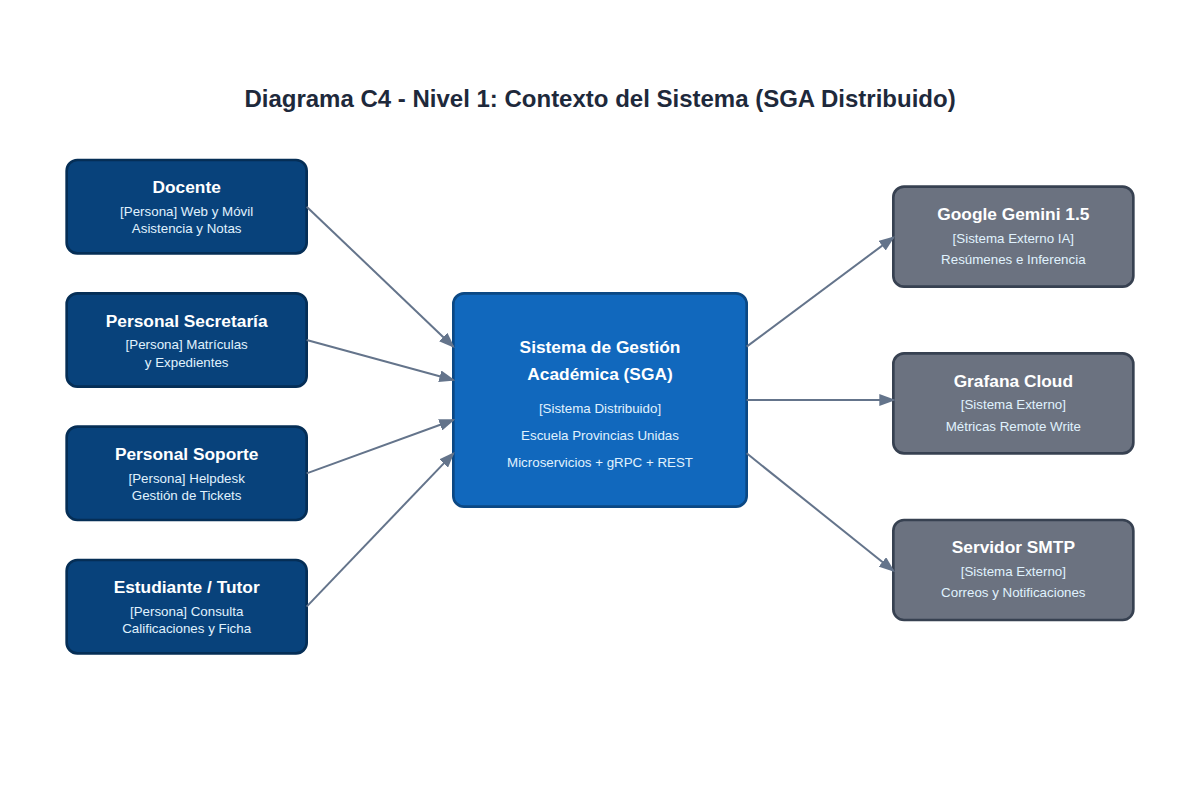
\includegraphics[width=0.82\textwidth]{c4_nivel1_contexto.png}
\caption{Diagrama C4 Nivel 1 -- Contexto del Sistema AcadTrace.}
\label{fig:c4-nivel1}
\end{figure}

\begin{figure}[H]
\centering
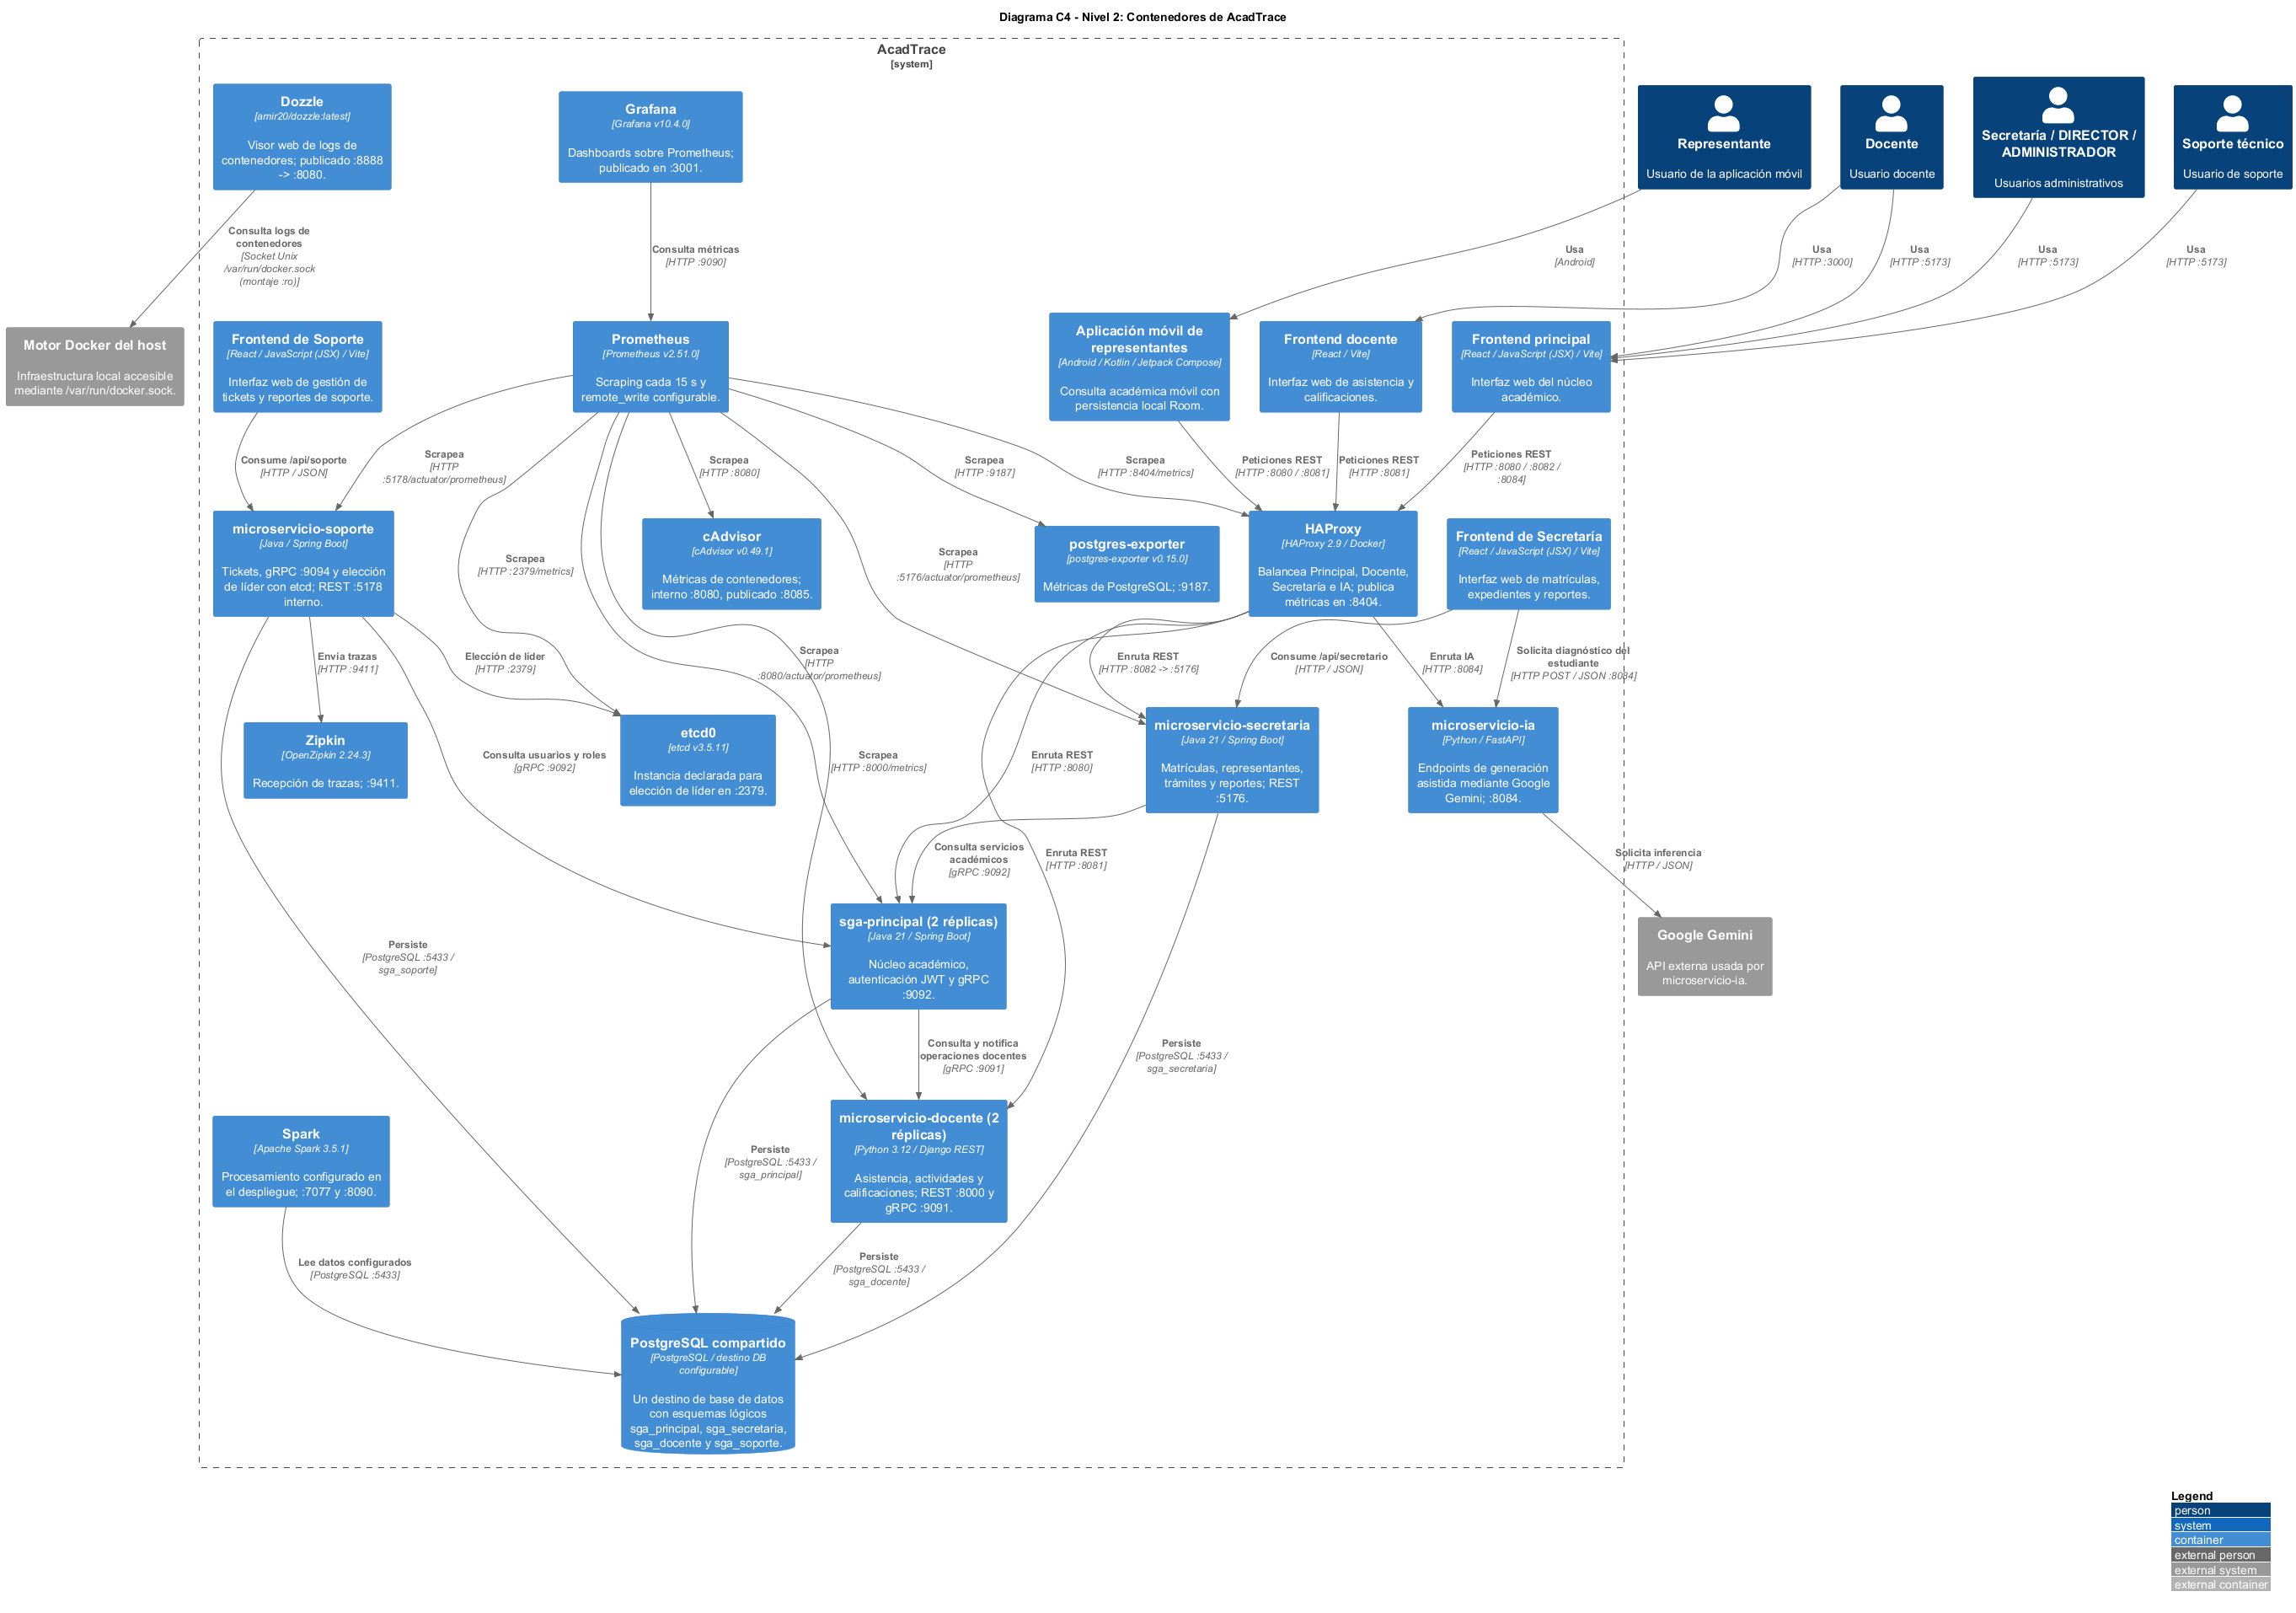
\includegraphics[width=0.88\textwidth]{c4_nivel2_contenedores.png}
\caption{Diagrama C4 Nivel 2 -- Contenedores, Puertos y Protocolos H\'ibridos.}
\label{fig:c4-nivel2}
\end{figure}

\begin{figure}[H]
\centering
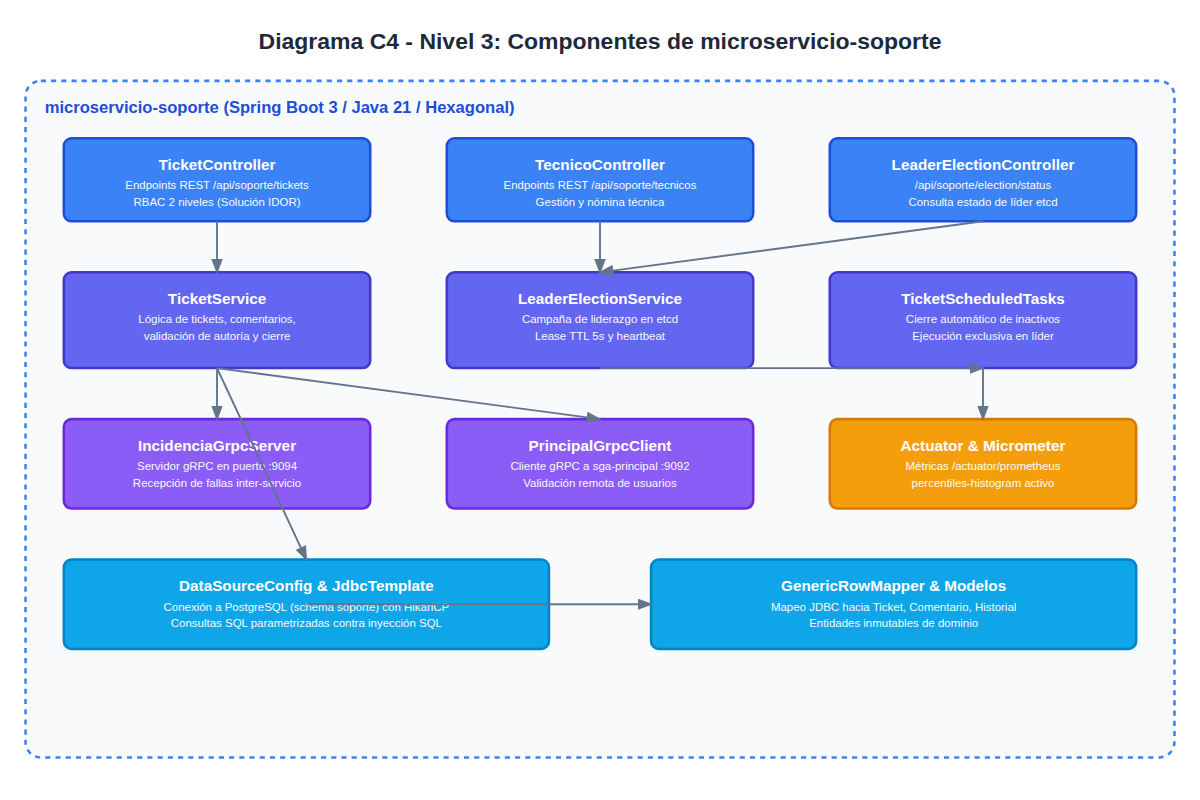
\includegraphics[width=0.88\textwidth]{c4_nivel3_componentes.png}
\caption{Diagrama C4 Nivel 3 -- Componentes Internos y Capas Hexagonales.}
\label{fig:c4-nivel3}
\end{figure}

\newpage

% =============================================================================
% 5. IMPLEMENTACIÓN DE APLICACIONES CLIENTE: WEB SPA Y MÓVIL
% =============================================================================

\subsection{Especificaci\'on de Servicios gRPC y Protocol Buffers v3}
Para viabilizar la sincronizaci\'on transaccional de alto rendimiento entre \texttt{sga-principal} y los microservicios sat\'elites, se compilaron definiciones de Protocol Buffers v3 (\texttt{asistencia.proto}, \texttt{actividades.proto}, \texttt{docente.proto}, \texttt{principal.proto}, \texttt{contexto\_docente.proto}). El Listing~\ref{lst:grpc-proto} ilustra la definici\'on del servicio de consulta y notificaci\'on de auditor\'ia:

\begin{lstlisting}[language=json, caption={Definici\'on Protobuf del canal sincr\'onico gRPC (\texttt{principal.proto}).}, label={lst:grpc-proto}]
syntax = "proto3";
package ec.edu.uteq.sga.grpc;

service PrincipalService {
  rpc ConsultarEstudiante (EstudianteRequest) returns (EstudianteResponse);
  rpc RegistrarCalificacionAuditable (CalificacionAuditableRequest) returns (AuditoriaResponse);
  rpc SincronizarEventosDocente (StreamEventosRequest) returns (SincronizacionResponse);
}

message CalificacionAuditableRequest {
  int64 id_matricula = 1;
  int64 id_asignatura = 2;
  double nota_formativa = 3;
  double nota_sumativa = 4;
  int64 lamport_clock = 5;
  string vector_clock_json = 6;
  string actor_id = 7;
}

message AuditoriaResponse {
  bool exitoso = 1;
  string hash_actual = 2;
  string hash_anterior = 3;
  int64 lamport_asignado = 4;
  string estado_reconciliacion = 5;
}
\end{lstlisting}

\subsection{Persistencia PostgreSQL y Separaci\'on L\'ogica Multiesquema}
\textbf{Persistencia de datos.} \texttt{docker-compose.yml} conecta los servicios a un mismo endpoint PostgreSQL parametrizado mediante variables de entorno \texttt{DB\_HOST}, \texttt{DB\_PORT} (predeterminado \texttt{5433}) y \texttt{DB\_NAME} (\texttt{sga}). No declara un servidor PostgreSQL. Como alternativa, \texttt{sga-principal/docker-compose.yml} declara una sola instancia \texttt{postgres:17}, con volumen persistente y puerto \texttt{5433:5432}; ambos Compose no constituyen un cl\'uster.

La configuraci\'on y los SQL versionados evidencian los esquemas \texttt{sga\_principal} (cat\'alogo, usuarios y auditor\'ia central), \texttt{sga\_docente} (calificaciones, actividades y asistencias), \texttt{sga\_secretaria} (estudiantes, representantes y matr\'iculas) y \texttt{sga\_soporte} (tickets y comentarios). Principal configura Flyway y Hibernate para \texttt{sga\_principal}; Docente usa \texttt{search\_path=sga\_docente,sga\_principal,public} y modelos con tablas en \texttt{sga\_docente}. Los SQL de Secretar\'ia y las migraciones de Soporte emplean los respectivos prefijos \texttt{sga\_}. Estos accesos no implican bases independientes ni exclusividad por servicio.

El SQL de referencia \texttt{docs/db/schema.sql} crea \texttt{sga\_principal}, \texttt{secretaria}, \texttt{docente} y \texttt{soporte}, con nombres distintos de los usados por los servicios. No demuestra su ejecuci\'on autom\'atica en los Compose ni sustituye la evidencia recogida en ADR-003. Tampoco se certifica la aplicaci\'on de todos los SQL al servidor externo. La separaci\'on por esquemas es l\'ogica: no se encontr\'o DDL de particiones por rango o lista en los SQL y migraciones revisados, y no garantiza eliminar bloqueos ni separar recursos de memoria y disco.

\textbf{Coordinaci\'on distribuida.} Soporte usa \texttt{LeaderElectionService}, la API Election de jetcd y leases sobre \texttt{/sga/leader} para condicionar las tareas de \texttt{TicketScheduledTasks} al liderazgo. Raft es interno a etcd y no replica PostgreSQL; esta coordinaci\'on no constituye un cl\'uster de persistencia. El Compose declara un servicio etcd.

\textbf{Limitaci\'on.} El repositorio no demuestra replicaci\'on PostgreSQL mediante Raft ni un cl\'uster de persistencia de tres nodos, standby o failover autom\'atico. La instancia \'unica y el endpoint compartido constituyen un punto \'unico de fallo de persistencia en la topolog\'ia evidenciada. La topolog\'ia interna y la versi\'on del servidor externo no se pueden certificar mediante estos archivos.

\subsection{Trazabilidad de Temas de la Asignatura y Evidencias del Proyecto}
\clearpage
\begin{table}[H]
\centering
\caption{Matriz de Trazabilidad: Temas de la Asignatura vs Implementaci\'on (Parte I: Arquitectura, Comunicaci\'on y Concurrencia).}
\label{tab:trazabilidad-temas-p1}
\scriptsize
\setlength{\tabcolsep}{3pt}
\renewcommand{\arraystretch}{1.02}
\begin{tabularx}{\textwidth}{|p{2.2cm}|p{2.5cm}|p{4.8cm}|c|p{1.4cm}|X|}
\hline
\textbf{Tema ISR-701} & \textbf{Mecanismo T\'ecnico} & \textbf{Archivo en Repositorio} & \textbf{L\'inea(s)} & \textbf{Autor} & \textbf{Qu\'e Demuestra / Verificaci\'on} \\
\hline
\textbf{1. Microservicios y SOLID} &
Clean Architecture en 4 capas conc\'entricas y cl\'uster pol\'iglota de 5 servicios. &
\texttt{sga-principal/src/main/java/}\allowbreak\texttt{ec/edu/uteq/sga/domain/}\allowbreak\texttt{entity/Estudiante.java} \newline
\texttt{docker-compose.yml} &
1--35 \newline
1--120 &
E. Luna, \newline P. Castro &
Aislamiento del dominio puro respecto a la infraestructura JPA; desacoplamiento en red bridge aislada. \\
\hline
\textbf{2. Patrones GoF Formalizados} &
Strategy, Template Method, Observer, Facade y Repository (ADR-005). &
\texttt{sga-principal/src/main/java/}\allowbreak\texttt{ec/edu/uteq/sga/domain/}\allowbreak\texttt{strategy/CalculoPromedioStrategy.java} &
1--28 &
P. Castro, \newline K. Bed\'on &
Intercambiabilidad de algoritmos de c\'alculo ponderado vs. simple y despacho desacoplado de eventos. \\
\hline
\textbf{3. gRPC y Protocol Buffers} &
Canal s\'incrono binario HTTP/2 con esquemas fuertemente tipados v3. &
\texttt{sga-principal/src/main/proto/}\allowbreak\texttt{principal.proto} \newline
\texttt{microservicio-docente/grpc\_protos/}\allowbreak\texttt{actividades.proto} &
1--45 \newline
1--40 &
K. Bed\'on, \newline P. Castro &
Interoperabilidad pol\'iglota Java-Python de alta eficiencia, validada en \texttt{test\_calificaciones\_grpc.py}. \\
\hline
\textbf{4. Relojes de Lamport} &
Reloj escalar mon\'otono creciente ($L = \max(L_{\text{loc}}, L_{\text{rx}}) + 1$). &
\texttt{sga-principal/src/main/java/}\allowbreak\texttt{ec/edu/uteq/sga/application/}\allowbreak\texttt{service/LamportClock.java} &
11--31 &
E. Luna, \newline P. Castro &
Ordenamiento causal determinista ante concurrencia sin dependencia de NTP; validado con pruebas unitarias. \\
\hline
\textbf{5. Relojes Vectoriales} &
Vectores l\'ogicos $\vec{V} = [v_1, \dots, v_n]$ para detecci\'on de causalidad ($A \parallel B$). &
\texttt{microservicio-docente/docentes/}\allowbreak\texttt{auditoria/clocks.py} &
11--47 &
K. Bed\'on &
Identificaci\'on de concurrencia en modo desconectado y algoritmo determinista \texttt{reconciliar\_vectores}. \\
\hline
\textbf{6. Balanceo con HAProxy} &
Reverse proxy perimetral con Round-Robin (REST), Leastconn (gRPC) y healthcheck. &
\texttt{infra/haproxy/haproxy.cfg} &
30--75 &
P. Castro, \newline E. Luna &
Distribuci\'on de carga hacia r\'eplicas activas, tolerancia a fallos (\texttt{fall 2 rise 2}) y m\'etricas en :8404. \\
\hline
\textbf{7. Sincronizaci\'on Offline-First} &
Persistencia SQLite Room con pol\'iticas de reintento y encolamiento en segundo plano. &
\texttt{app-movil-docente/app/src/main/}\allowbreak\texttt{java/.../sync/SyncWorker.kt} \newline
\texttt{RepresentanteSyncPolicy.kt} &
10--50 \newline
1--8 &
K. Bed\'on &
Disponibilidad desconectada de consultas de estudiantes/notas mediante \texttt{WorkManager} de Android. \\
\hline
\textbf{8. Capacidades de Dispositivo} &
Autenticaci\'on biom\'etrica de hardware nativa y canal de notificaciones push. &
\texttt{app-movil-docente/app/src/main/}\allowbreak\texttt{java/.../security/SecurityScreens.kt} &
23--45 &
K. Bed\'on &
Desbloqueo seguro con \texttt{BiometricPrompt} (\texttt{BIOMETRIC\_STRONG}) y gesti\'on de sesi\'on protegida. \\
\hline
\textbf{9. Pruebas de Contrato (Pact)} &
Verificaci\'on automatizada de contratos de interfaz cliente-proveedor sin simulacros. &
\texttt{microservicio-docente/tests/}\allowbreak\texttt{contract/test\_docente\_contract.py} &
1--55 &
K. Bed\'on &
Compatibilidad verificada de endpoints contra servidor real levantado en el propio proceso de ejecuci\'on. \\
\hline
\end{tabularx}
\end{table}

\clearpage
\begin{table}[H]
\centering
\caption{Matriz de Trazabilidad: Temas de la Asignatura vs Implementaci\'on (Parte II: Persistencia, Auditor\'ia, Resiliencia y Operaciones).}
\label{tab:trazabilidad-temas-p2}
\scriptsize
\setlength{\tabcolsep}{3pt}
\renewcommand{\arraystretch}{1.02}
\begin{tabularx}{\textwidth}{|p{2.2cm}|p{2.5cm}|p{4.8cm}|c|p{1.4cm}|X|}
\hline
\textbf{Tema ISR-701} & \textbf{Mecanismo T\'ecnico} & \textbf{Archivo en Repositorio} & \textbf{L\'inea(s)} & \textbf{Autor} & \textbf{Qu\'e Demuestra / Verificaci\'on} \\
\hline
\textbf{10. Particionamiento de Datos} &
Separaci\'on l\'ogica multiesquema en PostgreSQL por dominio. &
\texttt{docs/db/schema.sql} &
12--16 \newline
85--110 &
P. Castro, \newline K. Bed\'on &
SQL de referencia con esquemas; los nombres usados por servicios se detallan en ADR-003. No demuestra particiones f\'isicas ni eliminaci\'on de bloqueos. \\
\hline
\textbf{11. Auditor\'ia Criptogr\'afica} &
Encadenamiento SHA-256, hash de g\'enesis, hash anterior y bloqueo con \texttt{select\_for\_update}. &
\texttt{microservicio-docente/docentes/}\allowbreak\texttt{auditoria/strategies.py} \newline
\texttt{microservicio-docente/docentes/}\allowbreak\texttt{models.py} &
32--68 \newline
306--335 &
K. Bed\'on, \newline P. Castro &
Detecci\'on del 100\% ante manipulaci\'on directa en base de datos ($T_1$) o alteraci\'on de secuencia ($T_2$). \\
\hline
\textbf{12. Inmutabilidad Append-Only} &
Disparador PL/pgSQL a nivel de fila que rechaza sentencias UPDATE y DELETE. &
\path{sga-principal/src/main/resources/db/migration/V13__trigger_y_revocacion_auditoria.sql} \newline
\texttt{docs/db/schema.sql} &
11--26 \newline
156--170 &
E. Luna, \newline P. Castro &
Garant\'ia f\'isica de no-repudio; bloqueo estricto en el motor relacional PostgreSQL para registros de bit\'acora. \\
\hline
\textbf{13. Observabilidad Distribuida} &
Telemetr\'ia unificada con Prometheus (scrape 15\,s), cAdvisor y Grafana (6 vistas). &
\texttt{infra/prometheus/prometheus.yml} \newline
\texttt{ops/grafana/pfc-dashboard.json} &
13--55 \newline
1--120 &
J. Emanuel &
Monitoreo en tiempo real de RPS, percentiles de latencia (P50/P95/P99) y c\'odigos de error HTTP 4xx/5xx. \\
\hline
\textbf{14. PostgreSQL Exporter} &
Extracci\'on continua de telemetr\'ia del motor PostgreSQL para an\'alisis de conexiones. &
\texttt{docker-compose.yml} \newline
\texttt{infra/prometheus/prometheus.yml} &
85--95 \newline
45--55 &
J. Emanuel, \newline P. Castro &
Diagn\'ostico y monitoreo de saturaci\'on del pool de conexiones HikariCP y transacciones en base de datos. \\
\hline
\textbf{15. Consenso y Elecci\'on de L\'ider} &
Coordinaci\'on distribuida mediante \texttt{etcd}/Raft para alta disponibilidad en soporte. &
\texttt{microservicio-soporte/backend/}\allowbreak\texttt{src/main/java/.../election/}\allowbreak\texttt{LeaderElectionService.java} &
24--55 &
J. Emanuel &
Prevenci\'on de ejecuci\'on redundante de tareas programadas (\texttt{TicketScheduledTasks}) v\'ia leases sobre Raft. \\
\hline
\textbf{16. Procesamiento en Lotes} &
C\'alculo anal\'itico distribuido de promedios anuales y trimestrales con Apache Spark. &
\texttt{scripts/spark/}\allowbreak\texttt{calcular\_promedios\_anuales.py} \newline
\texttt{scripts/spark/common.py} &
1--65 \newline
1--45 &
K. Bed\'on, \newline P. Castro &
Procesamiento paralelo masivo batch con PySpark desacoplado de la carga transaccional de producci\'on. \\
\hline
\textbf{17. Pruebas de Carga (Locust)} &
Pruebas de estr\'es nominal (50 usuarios) con generaci\'on din\'amica de tokens JWT v\'alidos. &
\texttt{tests/load/locustfile.py} \newline
\texttt{generar\_evidencias.ps1} &
24--65 \newline
1--45 &
J. Emanuel, \newline P. Castro &
Evaluaci\'on emp\'irica de saturaci\'on bajo concurrencia real y verificaci\'on de seguridad en el API Gateway. \\
\hline
\textbf{18. Pipeline CI/CD} &
Flujo automatizado de 10 trabajos encadenados con construcci\'on, pruebas y Docker. &
\texttt{.github/workflows/ci-cd.yml} &
26--150 &
P. Castro &
Compilaci\'on integral de los 3 m\'odulos Java (196 pruebas), Python (83 pruebas) y empaquetado seguro. \\
\hline
\end{tabularx}
\end{table}
\clearpage

\newpage

\section{Aplicaciones Cliente: Portal Web SPA y Cliente M\'ovil Nativo}
\label{sec:clientes}

\subsection{M\'odulo B -- Aplicaci\'on Web SPA (React + TypeScript)}
El portal web est\'a construido en React 18 con Vite y Tailwind CSS, sirviendo las cinco rutas obligatorias protegidas por rol:
\begin{itemize}
  \item \texttt{/}: Dashboard institucional con m\'etricas en vivo de matr\'icula y asistencia.
  \item \texttt{/login}: Formulario de autenticaci\'on con generaci\'on de credencial JWT y almacenamiento en cookie HttpOnly/SessionStorage seguro.
  \item \texttt{/calificaciones}: M\'odulo principal de captura de calificaciones formativas/sumativas, c\'alculo en l\'inea con el patr\'on Strategy y emisi\'on de reportes PDF por per\'iodo lectivo.
  \item \texttt{/settings}: Configuraci\'on de par\'ametros institucionales, selecci\'on de tema (Claro / Oscuro) y selector de internacionalizaci\'on (Espa\~nol / Ingl\'es).
  \item \texttt{/about}: Ficha t\'ecnica de la versi\'on del sistema, estado del cl\'uster y metadatos de auditor\'ia.
\end{itemize}

Como evidencia operativa del cliente web para la gesti\'on administrativa, la Figura~\ref{fig:portal_secretaria} ilustra la interfaz del portal de Secretar\'ia (\texttt{localhost:5176/dashboard}). En dicho panel se centralizan las funciones administrativas del m\'odulo: estudiantes, grados y cursos, matr\'iculas, usuarios, promoci\'on, reportes, calendario, representantes, importaci\'on masiva e historial acad\'emico.

\begin{figure}[H]
\centering
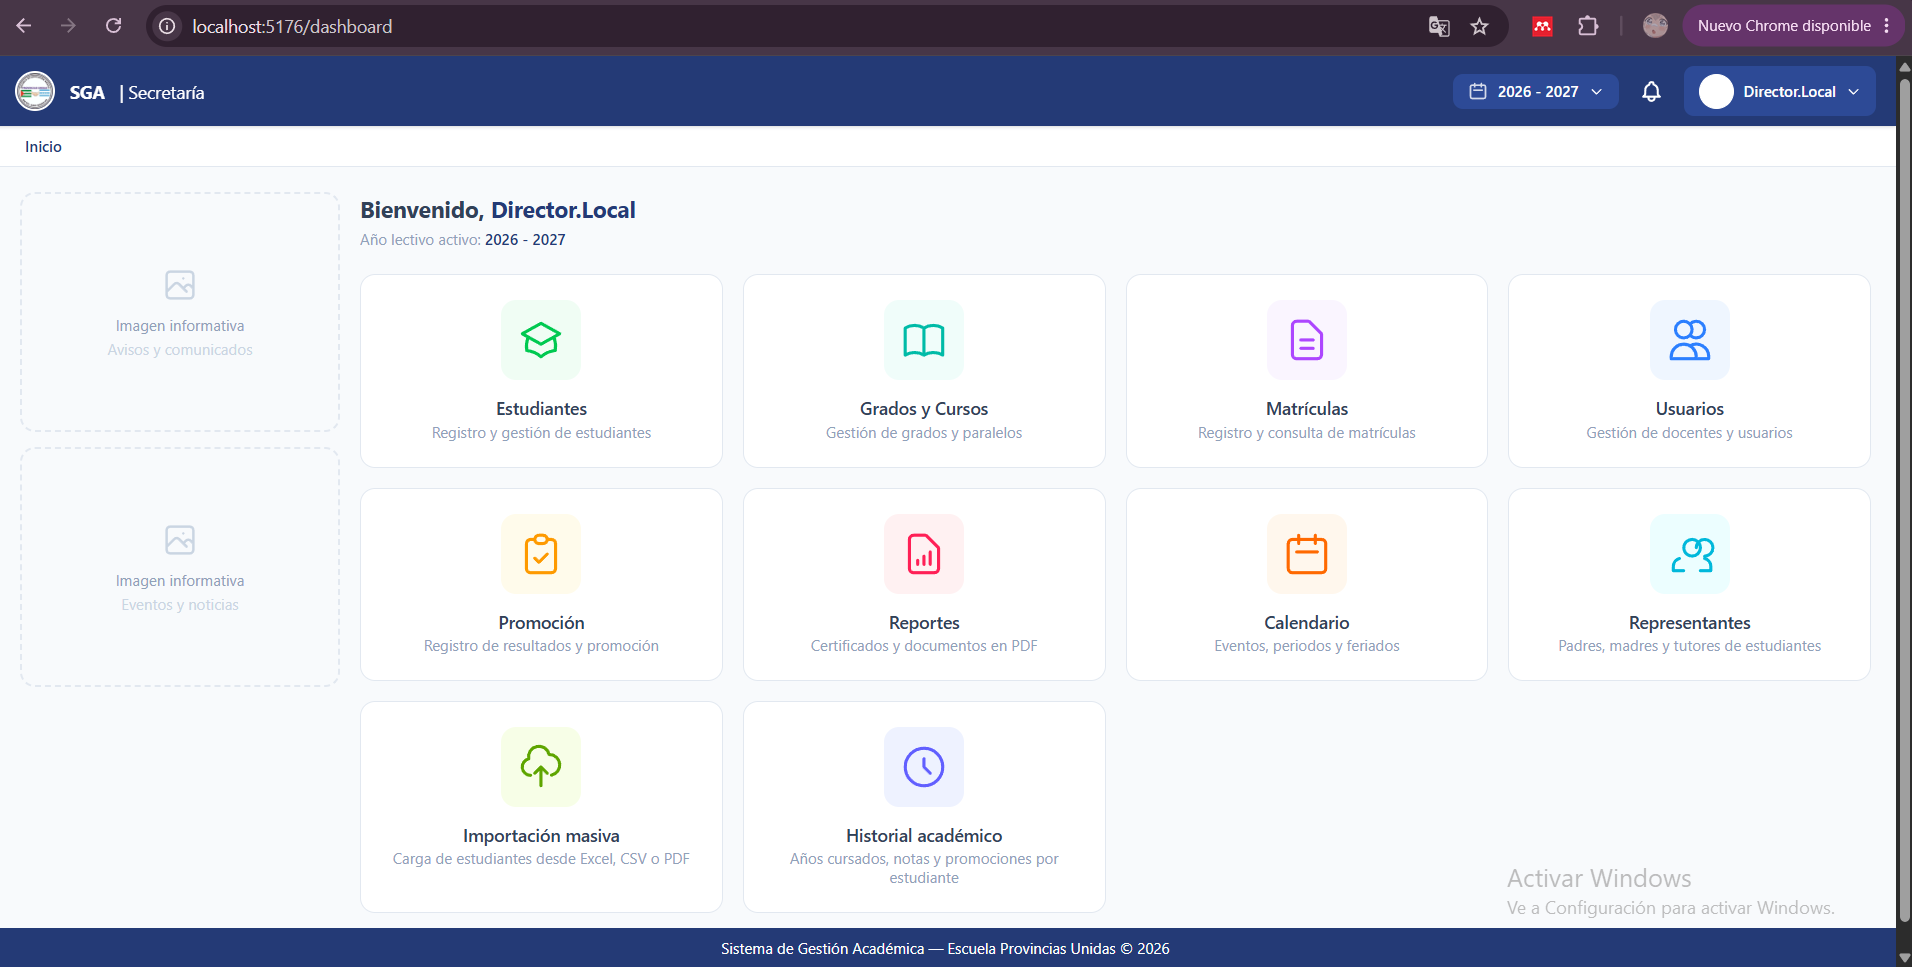
\includegraphics[width=0.88\textwidth]{secretaria_portal.png}
\caption{Portal web del m\'odulo de Secretar\'ia: panel de control administrativo con acceso a las funciones de estudiantes, grados y cursos, matr\'iculas, usuarios, promoci\'on, reportes, calendario, representantes, importaci\'on masiva e historial acad\'emico.}
\label{fig:portal_secretaria}
\end{figure}

Asimismo, como evidencia operativa de la gesti\'on de soporte t\'ecnico e incidencias, la Figura~\ref{fig:portal_soporte} ilustra el portal web del Microservicio de Soporte (\texttt{localhost:8083/soporte}). En dicha interfaz se visualiza el tablero interactivo de tickets estructurado bajo columnas de estado, destinado a la administraci\'on y seguimiento de requerimientos institucionales por parte del operador.

\begin{figure}[H]
\centering
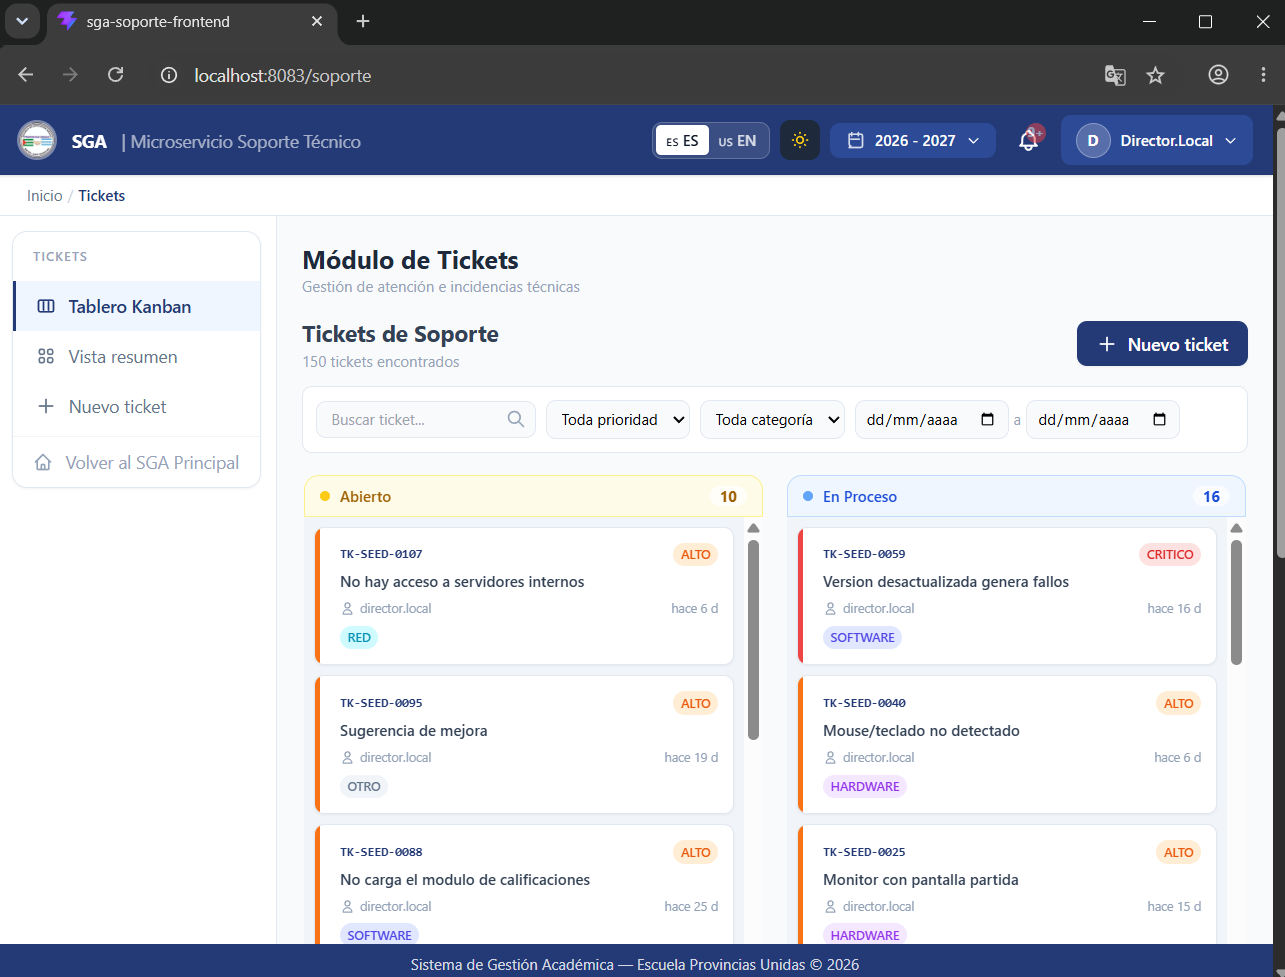
\includegraphics[width=0.88\textwidth]{soporte_tickets.png}
\caption{Portal web del Microservicio de Soporte: tablero interactivo de control para la administraci\'on y gesti\'on de incidencias con clasificaci\'on por estados de tickets.}
\label{fig:portal_soporte}
\end{figure}

\subsection{M\'odulo C -- Aplicaci\'on M\'ovil Nativa para Representantes (Kotlin + Jetpack Compose)}
La aplicaci\'on m\'ovil est\'a desarrollada en Android Nativo (SDK m\'inimo 26, objetivo 34) bajo arquitectura MVVM con soporte \textit{offline-first}:
\begin{enumerate}
  \item \textbf{Consulta de Calificaciones y Asistencia:} El representante visualiza en tiempo real el r\'ecord acad\'emico de su representado con gr\'aficas de progreso y desglose por quimestre/trimestre.
  \item \textbf{Capacidades del Dispositivo (Hardware):}
    \begin{itemize}
      \item \textbf{Notificaciones Push:} Gesti\'on con \texttt{NotificationManager} para alertar al representante de manera inmediata ante el registro de una nueva calificaci\'on o citaci\'on institucional.
      \item \textbf{Autenticaci\'on Biom\'etrica (\texttt{BiometricPrompt}):} Control de acceso criptogr\'afico mediante huella dactilar o reconocimiento facial para salvaguardar la privacidad de los expedientes de menores de edad.
    \end{itemize}
  \item \textbf{Sincronizaci\'on Desconectada:} Cach\'e local en base de datos SQLite (\texttt{Room}) con sincronizaci\'on en segundo plano gestionada por \texttt{WorkManager}.
\end{enumerate}

% =============================================================================
% 6. PIRÁMIDE DE PRUEBAS Y PIPELINE CI/CD
% =============================================================================

\subsection{Arquitectura por Caracter\'isticas y Seguridad de Sesi\'on en la Web SPA}
La aplicaci\'on web SPA implementa el patr\'on \textit{Feature-Based Architecture}, organizando el c\'odigo en m\'odulos cohesivos (\texttt{auth}, \texttt{grados}, \texttt{asignaciones}, \texttt{calificaciones}, \texttt{reportes}, \texttt{usuarios}). Cada m\'odulo encapsula sus propios componentes de interfaz, hooks personalizados de llamada a la API, servicios de transformaci\'on y modales de acci\'on.

En cumplimiento estricto de las directrices de seguridad de la Gu\'ia E4:
\begin{itemize}
  \item \textbf{Almacenamiento Seguro de Credenciales:} Los tokens JWT recibidos tras la autenticaci\'on en \texttt{/auth/login} no se almacenan en almacenamiento local plano (\texttt{localStorage}) para neutralizar ataques de \textit{Cross-Site Scripting} (XSS). Se gestionan mediante \texttt{sessionStorage} con expiraci\'on y cookies perimetrales protegidas con flags \texttt{HttpOnly}, \texttt{Secure} y \texttt{SameSite=Strict}.
  \item \textbf{Control de Acceso Basado en Roles (RBAC):} El enrutador de React (\texttt{react-router-dom}) protege las rutas sensibles (\texttt{/calificaciones}, \texttt{/settings}, \texttt{/reportes}) mediante un componente de orden superior (\texttt{ProtectedRoute}) que valida en memoria la firma y claims del token antes de renderizar la vista.
  \item \textbf{Internacionalizaci\'on Din\'amica y Tematizaci\'on:} El portal incorpora un hook de contexto (\texttt{ThemeLanguageContext}) que conmuta en tiempo de ejecuci\'on el diccionario de traducciones (\texttt{es.json} / \texttt{en.json}) y los esquemas crom\'aticos (\texttt{light} / \texttt{dark}) aplicando clases de Tailwind CSS sin recargar la p\'agina.
\end{itemize}

\subsection{Sincronizaci\'on Offline-First y Malla de Reconciliaci\'on en la App M\'ovil}
La aplicaci\'on m\'ovil nativa para Representantes resuelve el desaf\'io de conectividad intermitente mediante una arquitectura \textit{Offline-First} estructurada en tres capas locales:
\begin{enumerate}
  \item \textbf{Capa de Acceso a Datos Local (Room SQLite):} Tablas locales (\texttt{estudiantes\_cache}, \texttt{calificaciones\_cache}, \texttt{asistencias\_cache}, \texttt{cola\_pendientes}) decoradas con anotaciones JPA de Android Room para persistir las \'ultimas r\'ecas consultadas.
  \item \textbf{Cola Transaccional de Reintentos:} Cuando el dispositivo carece de conexi\'on a Internet, las solicitudes de justificaci\'on de faltas o confirmaci\'on de lectura de comunicados se encolan en \texttt{cola\_pendientes} con estado \texttt{PENDIENTE\_SINCRONIZACION} y marca de tiempo local.
  \item \textbf{Motor de Sincronizaci\'on en Background (\texttt{WorkManager}):} Un componente \texttt{Periodic\-Work\-Request\-Builder} con restricciones de red (\texttt{NetworkType.\allowbreak CONNECTED}) se activa autom\'aticamente al recuperar la conectividad, drenando la cola transaccional hacia el API Gateway mediante peticiones idempotentes y actualizando el reloj vectorial del dispositivo.
\end{enumerate}

La Figura~\ref{fig:app_movil_representante} reúne las vistas de seguridad, calificaciones y asistencia de la aplicación para representantes descrita en esta sección.

\begin{figure}[H]
\centering
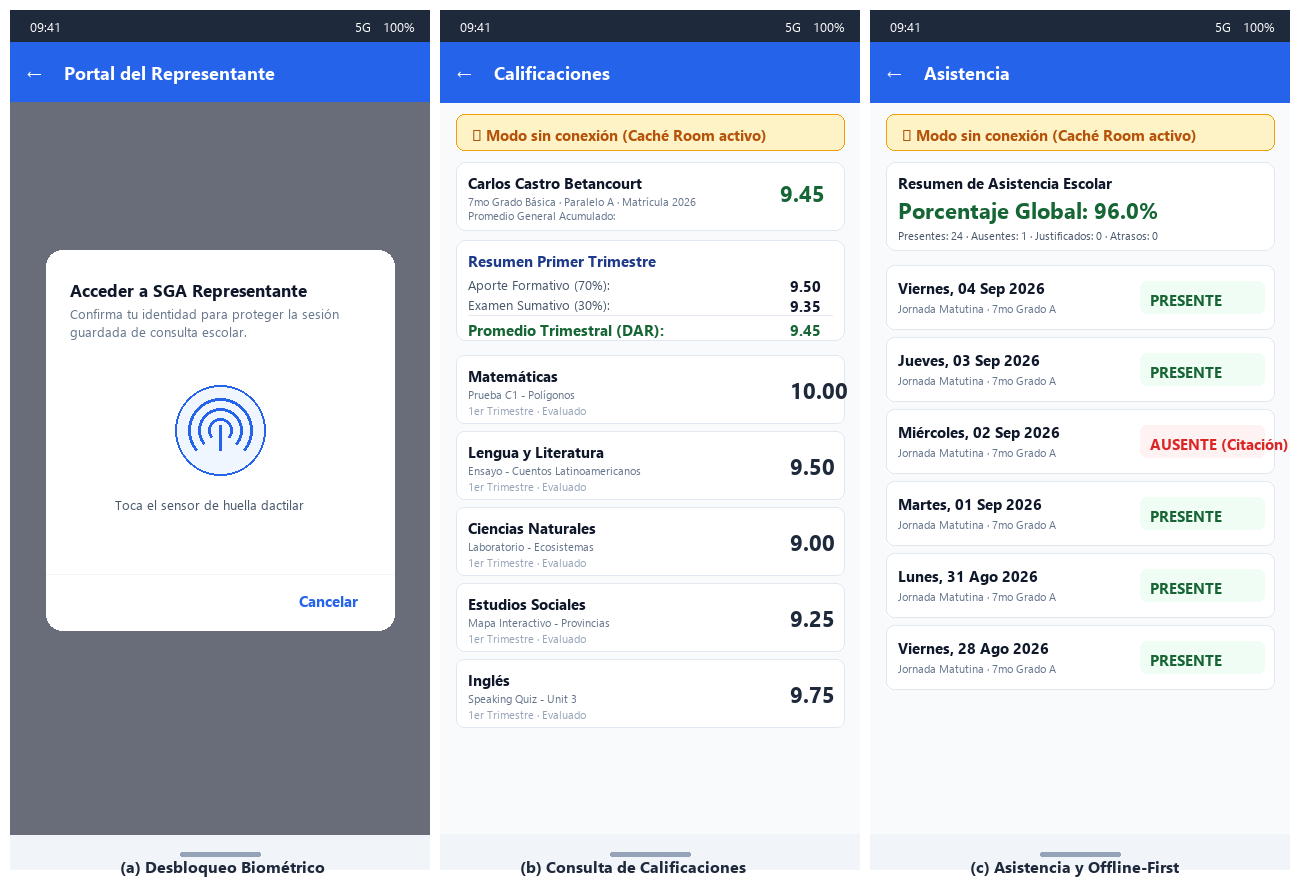
\includegraphics[width=0.88\textwidth]{movil_representante_evidencia.png}
\caption{Vistas reales de la Aplicaci\'on M\'ovil para Representantes (Kotlin + Jetpack Compose): (a) Configuraci\'on de seguridad y protecci\'on de acceso biom\'etrico, (b) Consulta de asignaturas y calificaciones trimestrales del estudiante representado, y (c) Resumen cuantitativo y consolidado de asistencia escolar categorizado por estados.}
\label{fig:app_movil_representante}
\end{figure}

\subsection{Evidencias visuales de interfaces y servicios}

El panel principal organiza los accesos a los módulos académicos y administrativos, como se observa en la Figura~\ref{fig:sga-principal}.

\begin{figure}[H]
    \centering
    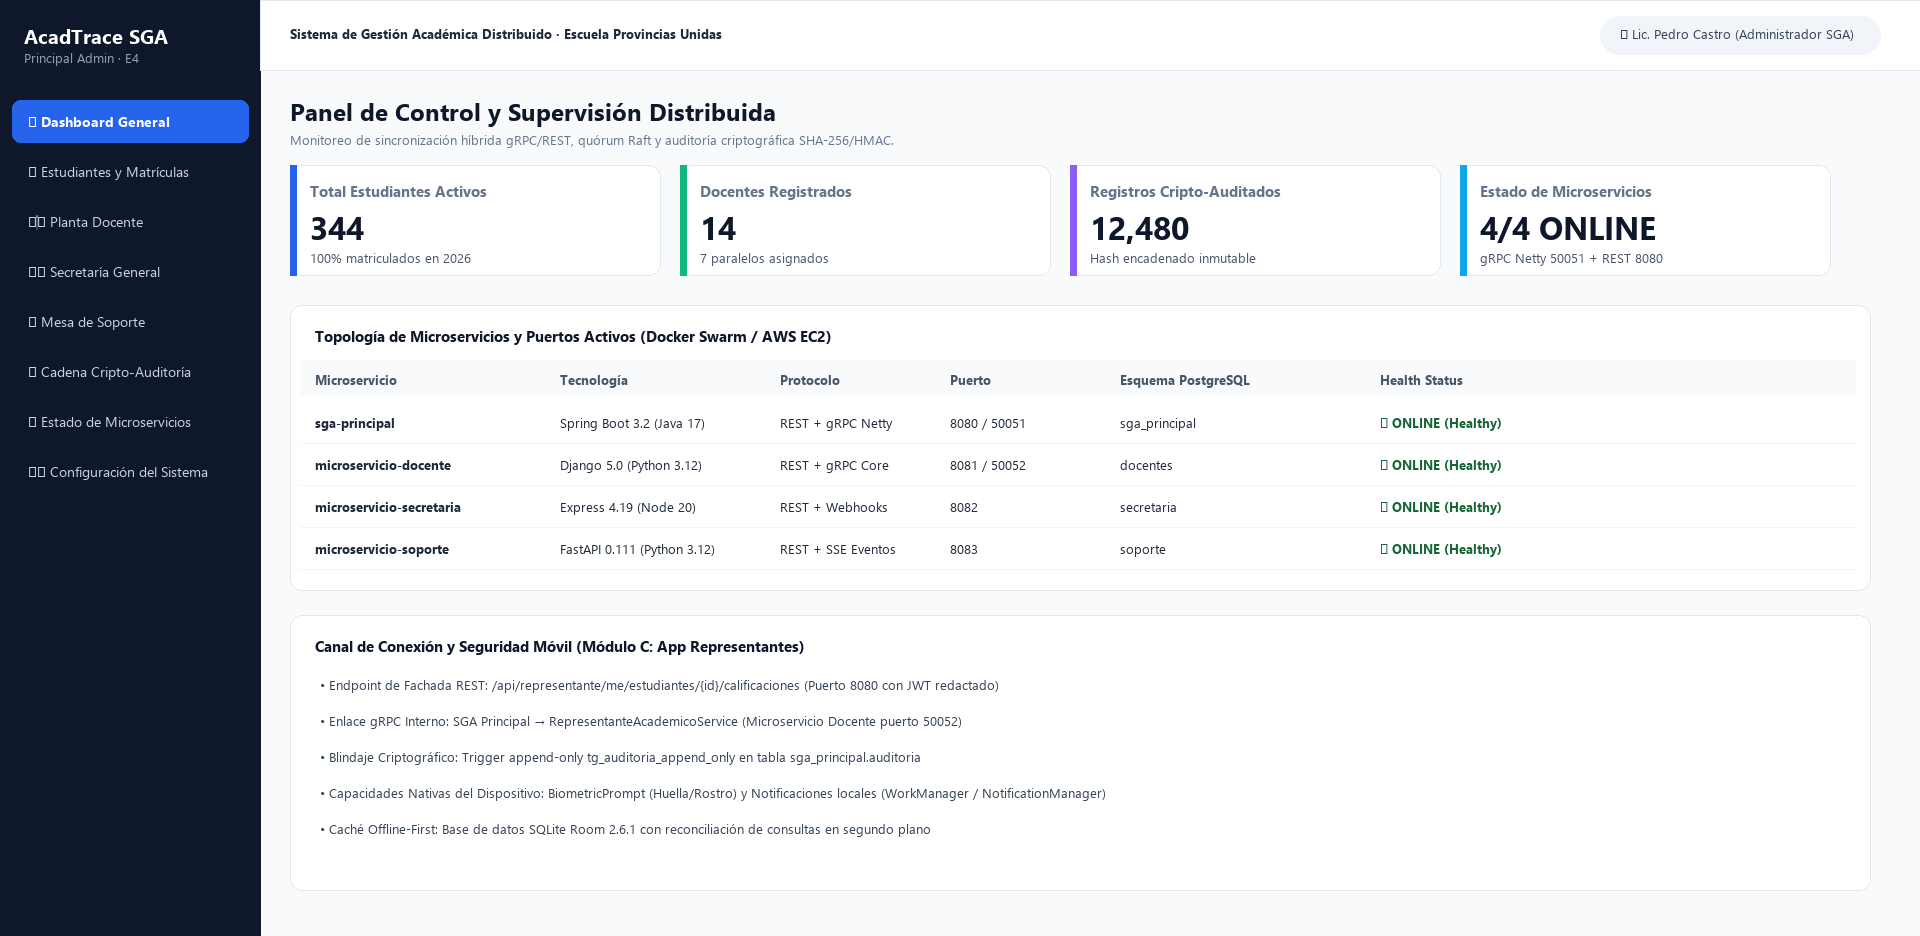
\includegraphics[width=0.88\textwidth]{../release/screenshots/sga_principal.png}
    \caption{Panel principal del SGA con accesos visibles a los m\'odulos acad\'emicos y administrativos.}
    \label{fig:sga-principal}
\end{figure}

La documentación de la API de IA presenta las rutas de salud, diagnóstico de estudiante y asistente en la Figura~\ref{fig:microservicio-ia}.

\begin{figure}[H]
    \centering
    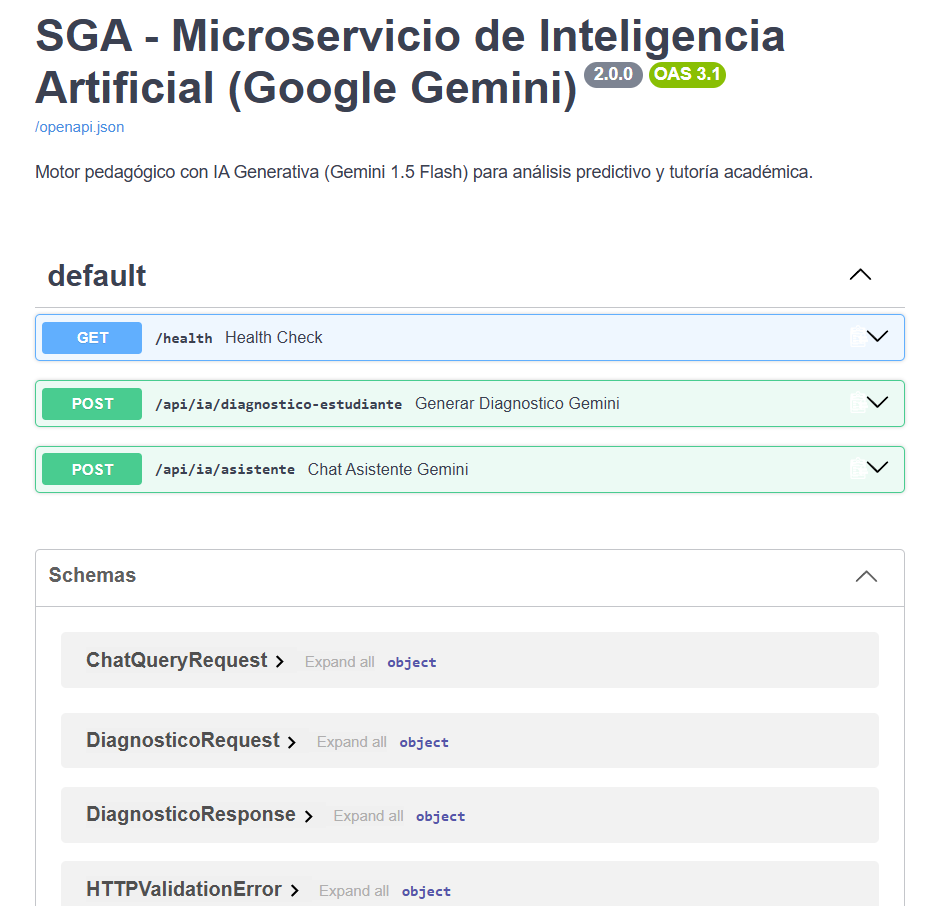
\includegraphics[width=0.88\textwidth]{../release/screenshots/microservicio_ia.png}
    \caption{Documentaci\'on de la API del microservicio de IA con las rutas de salud, diagn\'ostico de estudiante y asistente visibles.}
    \label{fig:microservicio-ia}
\end{figure}

En el portal docente, la vista de registro semanal permite seleccionar el curso y consultar los estados de asistencia por estudiante; la Figura~\ref{fig:docente-asistencia} muestra esta interfaz.

\begin{figure}[H]
    \centering
    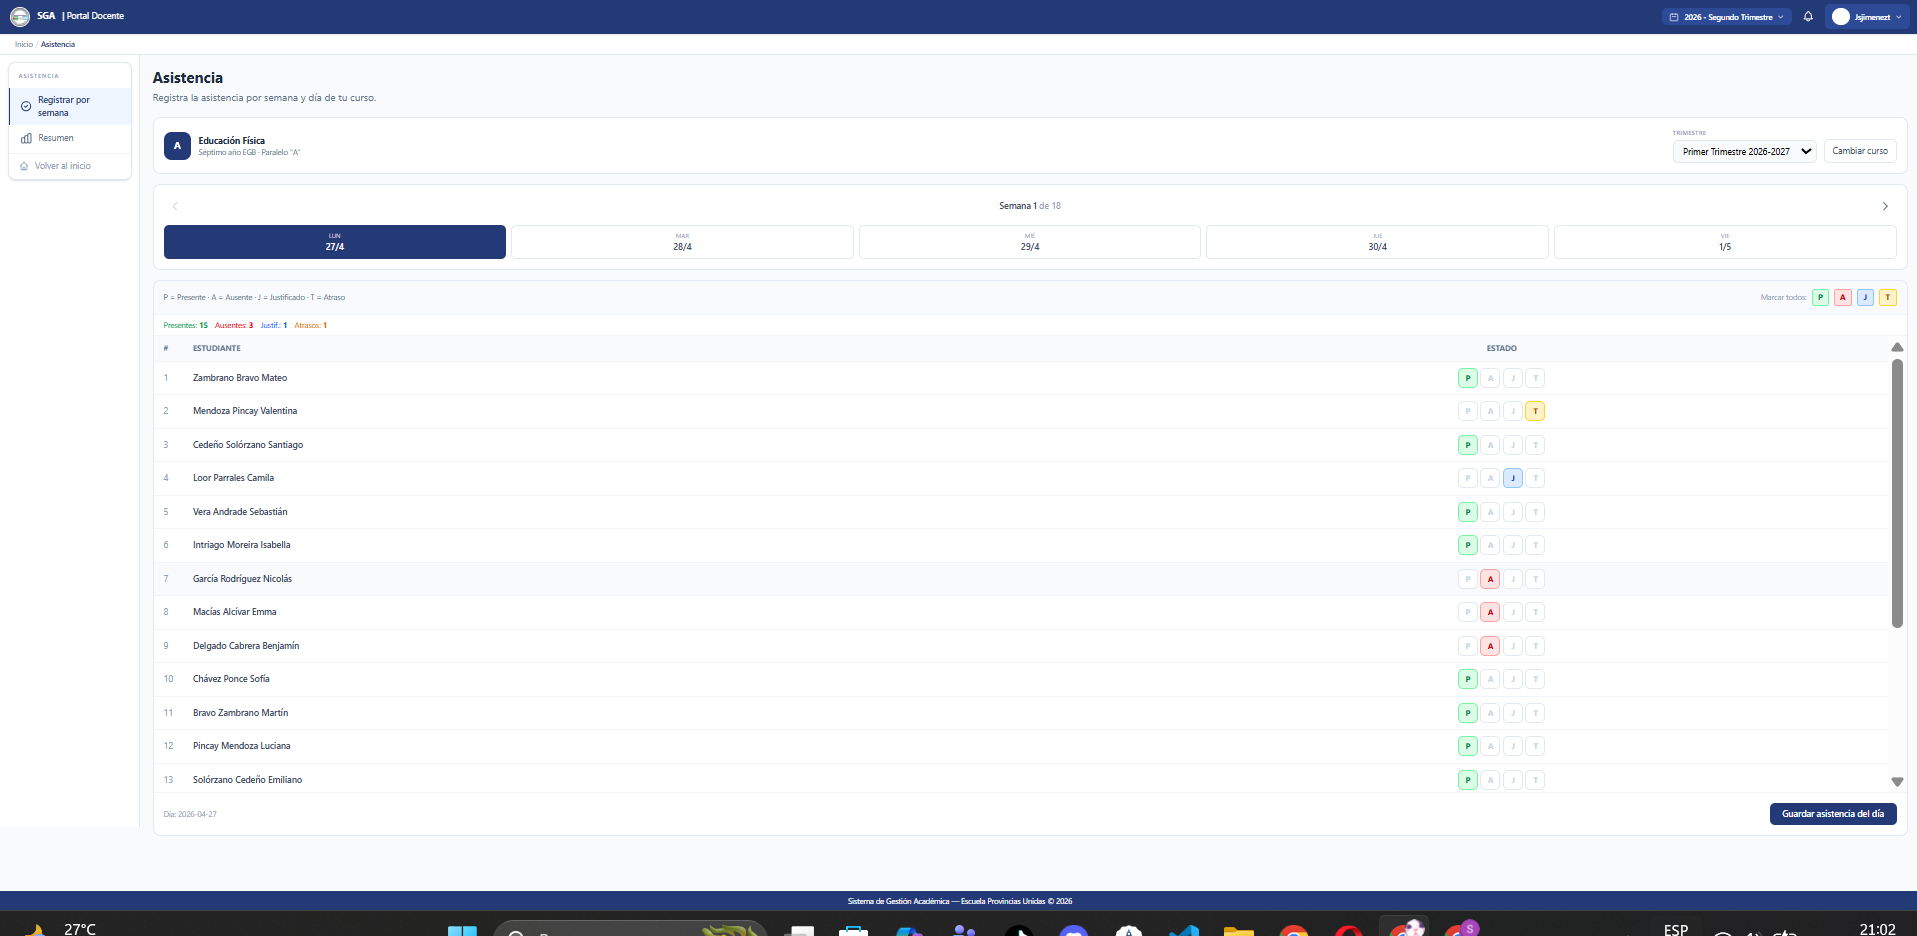
\includegraphics[width=0.88\textwidth]{../release/screenshots/docente_asistencia.png}
    \caption{Portal del docente en la vista de registro semanal de asistencia, con selecci\'on de curso y estados por estudiante.}
    \label{fig:docente-asistencia}
\end{figure}

En el cliente móvil, los ajustes de seguridad agrupan la protección de acceso y la opción de desbloqueo biométrico, visibles en la Figura~\ref{fig:movil-biometria}.

\begin{figure}[H]
    \centering
    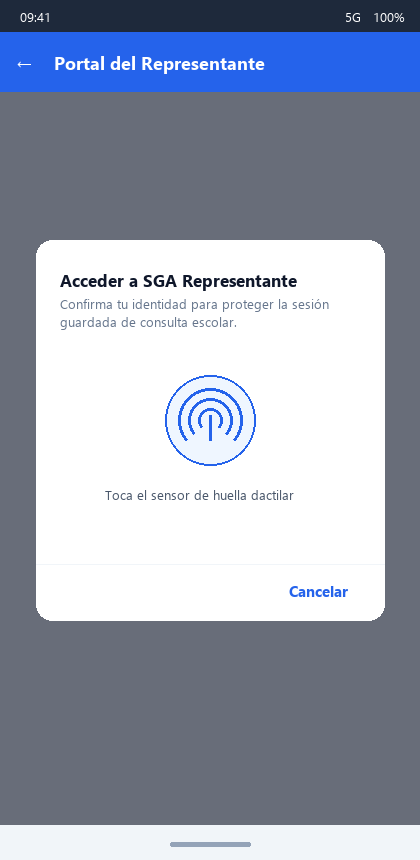
\includegraphics[width=0.52\textwidth]{../release/screenshots/movil_representante_biometria.png}
    \caption{Aplicaci\'on m\'ovil del representante: pantalla de ajustes de seguridad con gesti\'on de protecci\'on, interruptor para desbloqueo biom\'etrico y avisos de expiraci\'on de sesi\'on.}
    \label{fig:movil-biometria}
\end{figure}

La consulta de calificaciones del representante organiza las asignaturas y sus ponderaciones por trimestre, como muestra la Figura~\ref{fig:movil-calificaciones}.

\begin{figure}[H]
    \centering
    
\includegraphics[width=0.52\textwidth]{../release/screenshots/movil_representante_calificaciones.png}
    \caption{Aplicaci\'on m\'ovil del representante: vista de calificaciones detalladas por trimestre con listado de asignaturas y ponderaciones.}
    \label{fig:movil-calificaciones}
\end{figure}

El resumen de asistencia complementa la consulta académica con el desglose por estados mostrado en la Figura~\ref{fig:movil-asistencia}.

\begin{figure}[H]
    \centering
    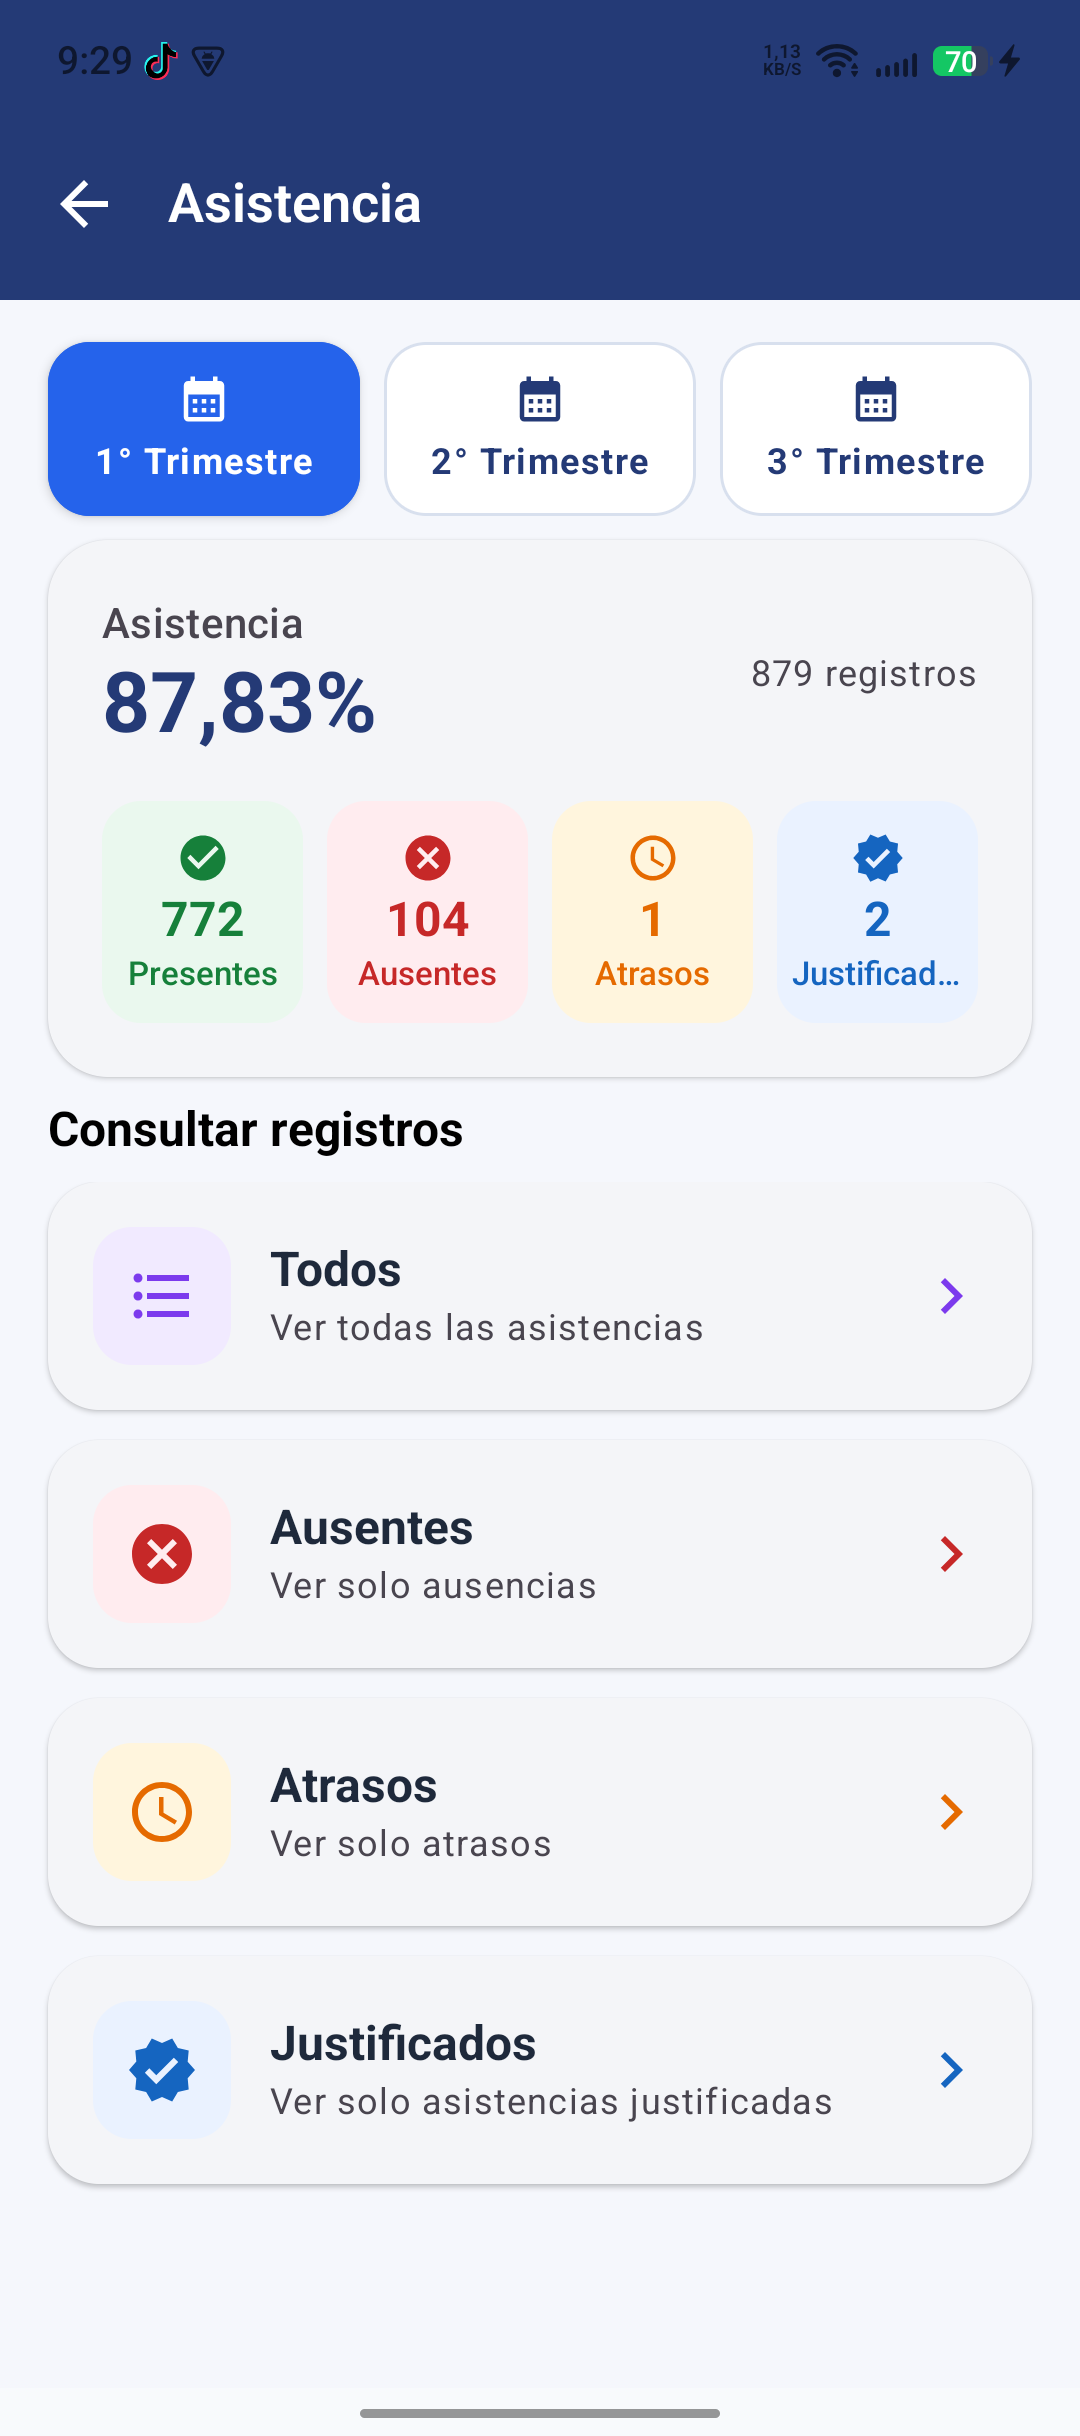
\includegraphics[width=0.52\textwidth]{../release/screenshots/movil_representante_asistencia.png}
    \caption{Aplicaci\'on m\'ovil del representante: resumen porcentual global de asistencia (87,83\,\%) y desglose interactivo por categor\'ias (presentes, ausentes, atrasos y justificados).}
    \label{fig:movil-asistencia}
\end{figure}

% =============================================================================
% 6. PIRÁMIDE DE PRUEBAS Y PIPELINE CI/CD
% =============================================================================
\label{sec:pruebas-cicd}

\subsection{Pir\'amide de Pruebas de Cinco Niveles}
La estrategia de aseguramiento de calidad cubre los cinco estratos exigidos:
\begin{enumerate}
  \item \textbf{Unitarias:} Evidencia conservada de pruebas de servicios con dobles de prueba (Mockito en Java, \texttt{pytest-mock} en Python): Cobertura oficial JaCoCo del m\'odulo \texttt{sga-principal}: 32,79\,\% de instrucciones (4668/14237) sobre el BUNDLE completo (excluyendo c\'odigo generado gRPC, DTOs, entidades JPA y configuraci\'on Spring). Compuerta CI configurada al 30\,\% m\'inimo con \texttt{<element>BUNDLE</element>} en \texttt{pom.xml}.
  \item \textbf{Integraci\'on:} Validaci\'on de repositorios y transacciones con aislamiento de esquemas.
  \item \textbf{Contrato:} Pruebas con \textbf{Pact} (\texttt{portal-docente-microservicio-docente.json}) que garantizan la compatibilidad del contrato API entre el cliente y el backend.
  \item \textbf{Extremo a Extremo (E2E):} Verificaci\'on de flujos completos desde la autenticaci\'on hasta la consulta de datos.
  \item \textbf{Carga y Estr\'es:} Pruebas automatizadas con \textbf{Locust} bajo dos escenarios obligatorios:
    \begin{itemize}
      \item \textit{Escenario 1 (Carga Nominal):} 50 usuarios concurrentes durante 5 minutos.
      \item \textit{Escenario 2 (Estr\'es / Cierre de Per\'iodo):} Rampa progresiva de 0 a 200 usuarios concurrentes durante 10 minutos.
    \end{itemize}
\end{enumerate}

Como evidencia complementaria de observabilidad, la Figura~\ref{fig:grafana-hikari-latencias} muestra el panel de Grafana con métricas del pool HikariCP y percentiles de latencia; corresponde a una captura histórica, no a la interfaz de Locust.

\begin{figure}[H]
\centering
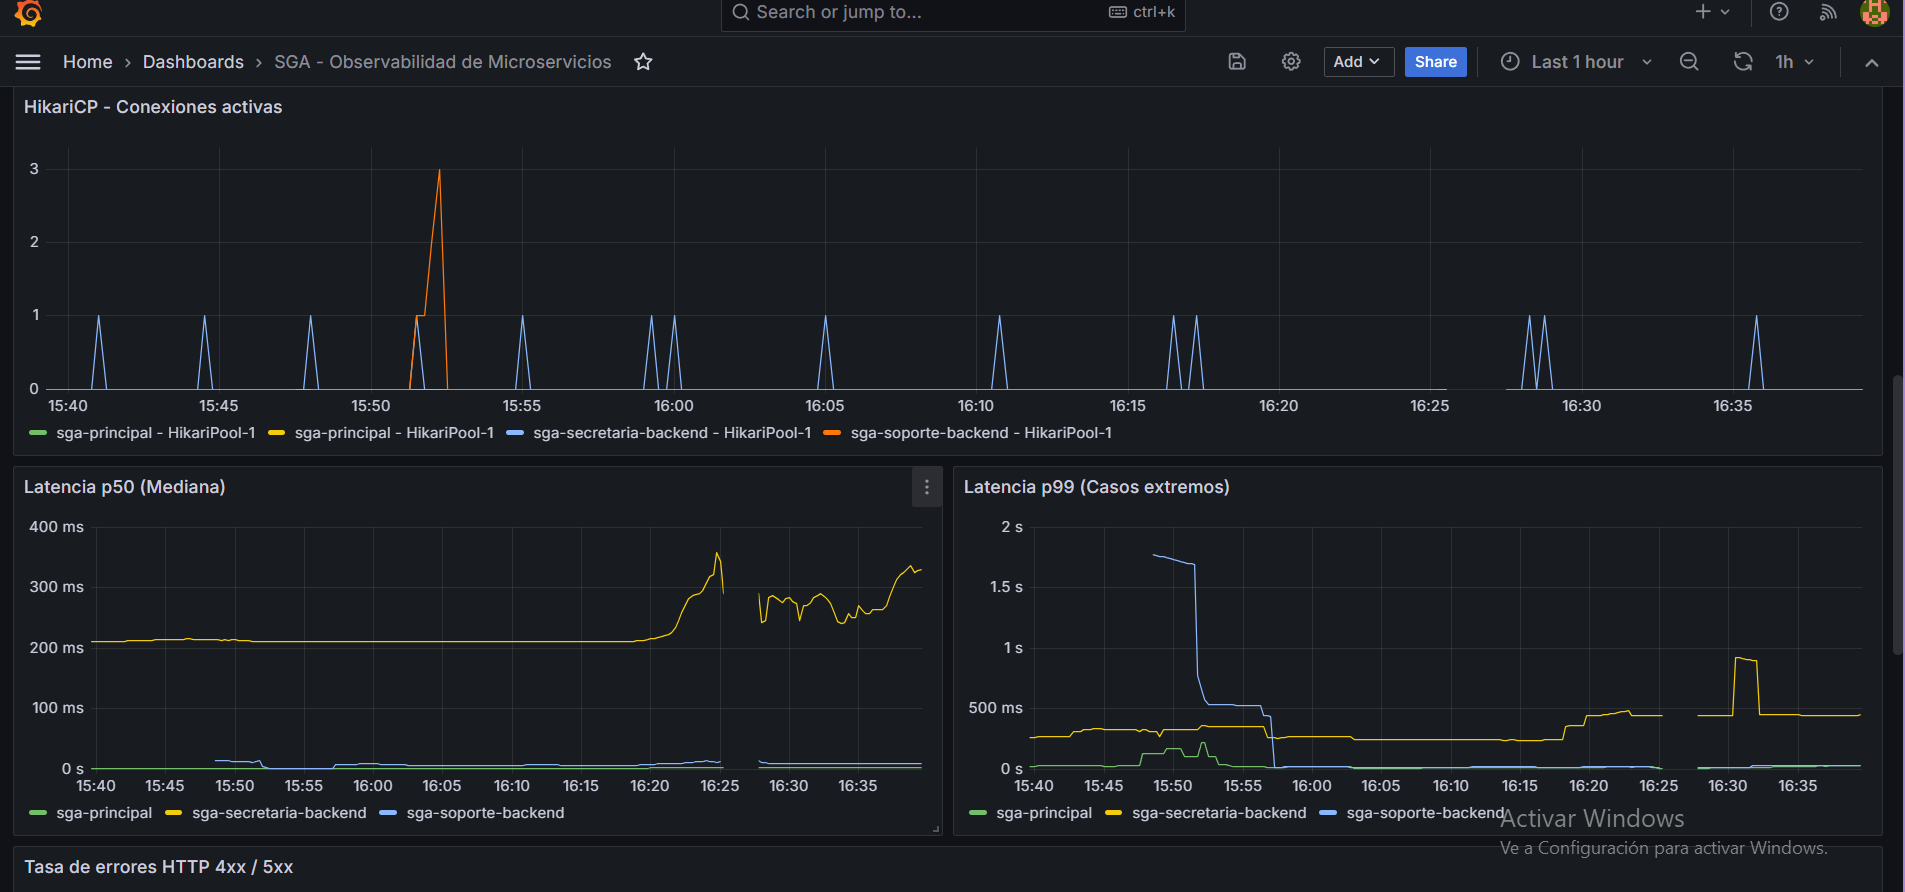
\includegraphics[width=0.85\textwidth]{grafana_hikari_p95.png}
\caption{M\'etricas de observabilidad en Grafana durante la ejecuci\'on de pruebas de carga: monitoreo del pool HikariCP y percentiles de latencia ($P_{50}$ y $P_{99}$) como evidencia complementaria.}
\label{fig:grafana-hikari-latencias}
\end{figure}

\subsection{Pipeline CI/CD de Siete Trabajos Encadenados (GitHub Actions)}
\label{subsec:pipeline-cicd}
El archivo \texttt{.github/workflows/ci-cd.yml} orquesta siete trabajos bloqueantes ejecutados de forma totalmente automatizada ante cada evento de \textit{push} o \textit{pull request} hacia la rama \texttt{main}:

\begin{table}[H]
\centering
\caption{Estructura y Responsabilidades de los Siete Trabajos del Pipeline CI/CD.}
\label{tab:pipeline-jobs}
\small
\begin{tabular}{|l|l|p{8.5cm}|}
\hline
\textbf{Orden} & \textbf{Job ID} & \textbf{Funci\'on y Validaci\'on Ejecutada} \\
\hline
1 & \texttt{lint} & An\'alisis est\'atico con Flake8 y validaci\'on de formato en Python y Java. \\
\hline
2 & \texttt{test-backend} & Tests unitarios Java (Surefire/JaCoCo con umbrales configurados por m\'odulo en Maven) y Python (\texttt{pytest-cov} al 70\,\%); el umbral es criterio de calidad, no resultado medido. \\
\hline
3 & \texttt{test-web} & Compilaci\'on TypeScript y empaquetado de distribuciones React en \texttt{.tar.gz}. \\
\hline
4 & \texttt{test-mobile} & Ejecuci\'on de pruebas unitarias JVM de Android (\texttt{testDebugUnitTest}). \\
\hline
5 & \texttt{build-images} & Construcci\'on y publicaci\'on de im\'agenes en GHCR (\texttt{ghcr.io/...:sha}). \\
\hline
6 & \texttt{build-mobile-apk} & Compilaci\'on, firma y verificaci\'on del APK/AAB de release; ante un tag de versi\'on v\'alido, publicaci\'on autom\'atica de los artefactos y sus sumas SHA-256 en GitHub Release. \\
\hline
7 & \texttt{integration} & Despliegue seguro v\'ia SSH a AWS EC2 condicionado al \'exito de los 6 jobs previos. \\
\hline
\end{tabular}
\end{table}

\subsection{Cultura DevOps, Shift-Left Testing y Sintaxis Declarativa YAML}
\label{subsec:devops-yaml}
La adopci\'on de la cultura DevOps en AcadTrace se fundamenta en el marco conceptual CALMS (\textit{Culture, Automation, Lean, Measurement, Sharing}), enfatizando la pr\'actica de \textbf{\textit{Shift-Left Testing}}, mediante la cual las compuertas de verificaci\'on est\'atica, pruebas unitarias y validaci\'on de cobertura se desplazan hacia las fases m\'as tempranas del ciclo de desarrollo:

\begin{itemize}[leftmargin=*]
  \item \textbf{Directiva \texttt{name} y Eventos Desencadenadores (\texttt{on}):} Define el identificador legible del flujo y los eventos que activan el pipeline (\texttt{push}, \texttt{pull\_request}) filtrados por ramas objetivo (\texttt{branches: [main]}).
  \item \textbf{Ambientes de Ejecuci\'on (\texttt{runs-on}):} Cada trabajo se ejecuta en un contenedor virtualizado aislado (\texttt{ubuntu-latest}), garantizando reproducibilidad e independencia de entorno.
  \item \textbf{Matriz de Dependencias (\texttt{needs}):} Modela el grafo ac\'iclico dirigido (DAG) de dependencias entre trabajos, impidiendo que el despliegue (\texttt{integration}) se ejecute si alguno de los trabajos de prueba previos (\texttt{lint}, \texttt{test-backend}, \texttt{test-web}, \texttt{test-mobile}) falla.
  \item \textbf{Composici\'on de Pasos (\texttt{steps}, \texttt{uses}, \texttt{with}, \texttt{run}):} Articula la secuencia de acciones reutilizando acciones comunitarias auditadas (\texttt{actions/\allowbreak checkout@v4}, \texttt{actions/\allowbreak setup-java@v4}, \texttt{docker/\allowbreak build-push-action@v5}) combinadas con scripts de compilaci\'on deterministas.
  \item \textbf{Gesti\'on Segura de Secretos (\texttt{secrets.*}):} Variables cr\'iticas como llaves privadas SSH, tokens de GitHub Container Registry (GHCR) y credenciales de AWS no se exponen en c\'odigo plano, siendo inyectadas en memoria durante la ejecuci\'on.
\end{itemize}

\subsection{Estrategias de Despliegue en Sistemas Distribuidos}
\label{subsec:estrategias-despliegue}
Para mitigar el riesgo de indisponibilidad durante las actualizaciones de los microservicios en producci\'on, se analizaron tres patrones de despliegue continuo:

\begin{enumerate}[leftmargin=*]
  \item \textbf{Despliegue Blue-Green (\textit{Blue-Green Deployment}):} Mantiene dos entornos de producci\'on id\'enticos pero aislados. Mientras el entorno \textit{Blue} atiende el tr\'afico activo, la nueva versi\'on se despliega en \textit{Green}. Tras superar las pruebas de salud, el balanceador perimetral HAProxy conmuta el 100\% del tr\'afico hacia \textit{Green} de forma instant\'anea ($< 1$\,s), permitiendo un retorno inmediato (\textit{rollback}) ante anomal\'ias.
  \item \textbf{Despliegue Canario (\textit{Canary Releases}):} Enruta progresivamente una fracci\'on controlada del tr\'afico (e.g., 5\% $\to$ 25\% $\to$ 100\%) hacia las nuevas instancias del microservicio. Permite monitorear m\'etricas de latencia y tasa de errores 5xx en Prometheus antes de impactar a la totalidad de la poblaci\'on estudiantil.
  \item \textbf{Actualizaci\'on Rodante (\textit{Rolling Update}):} Reemplaza secuencialmente las r\'eplicas de los contenedores una a una dentro del cl\'uster Docker Compose / Kubernetes, manteniendo la capacidad de atenci\'on sin tiempos de inactividad (\textit{zero-downtime}).
\end{enumerate}

\newpage

% =============================================================================
% 7. OBSERVABILIDAD DISTRIBUIDA
% =============================================================================
\section{Observabilidad Distribuida y Monitoreo en Tiempo Real}
\label{sec:observabilidad}
La observabilidad se articula mediante la recolecci\'on de m\'etricas de Prometheus cada 15 segundos, recolecci\'on de recursos de contenedores con cAdvisor y un tablero de Grafana (\texttt{ops/\allowbreak grafana/\allowbreak pfc-dashboard.json}) estructurado en seis vistas:

\begin{enumerate}
  \item \textbf{Vista 1 (Tasa de Peticiones - RPS):} Throughput discriminado por microservicio y tr\'afico global en HAProxy.
  \item \textbf{Vista 2 (Latencias Percentiles P50, P95, P99):} Detecci\'on de colas de latencia bajo concurrencia.
  \item \textbf{Vista 3 (Tasa de Errores 4xx / 5xx):} Ratio de rechazo por autenticaci\'on frente a fallas de servidor.
  \item \textbf{Vista 4 (Disponibilidad y Consenso Raft):} Estado del l\'ider de consenso y conexiones HikariCP.
  \item \textbf{Vista 5 (Uso de CPU y RAM por Contenedor):} M\'etricas provistas por cAdvisor para prevenir sobrecargas.
  \item \textbf{Vista 6 (Latencia E2E Cliente M\'ovil):} Tiempos de respuesta de extremo a extremo desde el dispositivo m\'ovil.
\end{enumerate}

\subsection{M\'etricas de Negocio de Aplicaci\'on (Equipo BCEL)}
En cumplimiento de la secci\'on 4.6 de la gu\'ia rectora para el Equipo BCEL, la instrumentaci\'on de Prometheus incluye cuatro contadores obligatorios de eventos cr\'iticos de dominio:
\begin{enumerate}
  \item \textbf{Notas registradas (\texttt{sga\_notas\_registradas\_total}):} Total acumulado de calificaciones formativas y sumativas ingresadas por los docentes.
  \item \textbf{Notas modificadas (\texttt{sga\_notas\_modificadas\_total}):} Total de rectificaciones de calificaciones, disparando el siguiente eslab\'on criptogr\'afico de auditor\'ia.
  \item \textbf{Matr\'iculas confirmadas (\texttt{sga\_matriculas\_confirmadas\_total}):} Registro acumulado de legalizaci\'on de matr\'iculas para la poblaci\'on de 344 estudiantes.
  \item \textbf{Notificaciones enviadas a representantes (\texttt{sga\_notificaciones\_representantes\_total}):} Total de alertas y avisos emitidos hacia la aplicaci\'on m\'ovil.
\end{enumerate}
Estos contadores alimentan las vistas del tablero en Grafana y constituyen la base emp\'irica para evaluar el comportamiento transaccional del sistema.

\subsection{Registro Estructurado JSON y Propagaci\'on de Contexto MDC}
Para garantizar la correlaci\'on de eventos transaccionales a lo largo de m\'ultiples saltos de red, se implement\'o un filtro de trazabilidad (\texttt{TraceIdFilter}) y un contenedor de contexto (\texttt{TraceContext}) en los microservicios Java y Python. Cada petici\'on entrante recibe o genera un identificador \'unico de correlaci\'on (\texttt{trace\_id}) que es inyectado en el \textit{Mapped Diagnostic Context} (MDC) de SLF4J / Logback y en los encabezados binarios de las llamadas gRPC.

El layout personalizado \texttt{JsonStructuredLayout} formatea los registros en JSON emitidos por consola estándar (\texttt{stdout}), incluyendo los campos: \texttt{timestamp}, \texttt{level}, \texttt{service}, \texttt{trace\_id}, \texttt{thread}, \texttt{logger} y \texttt{message}. La emisi\'on estructurada es validada autom\'aticamente mediante pruebas unitarias (\texttt{JsonLoggingTest} y \texttt{test\_observability.py}) que comprueban la presencia ininterrumpida de estos campos.

\begin{figure}[H]
\centering
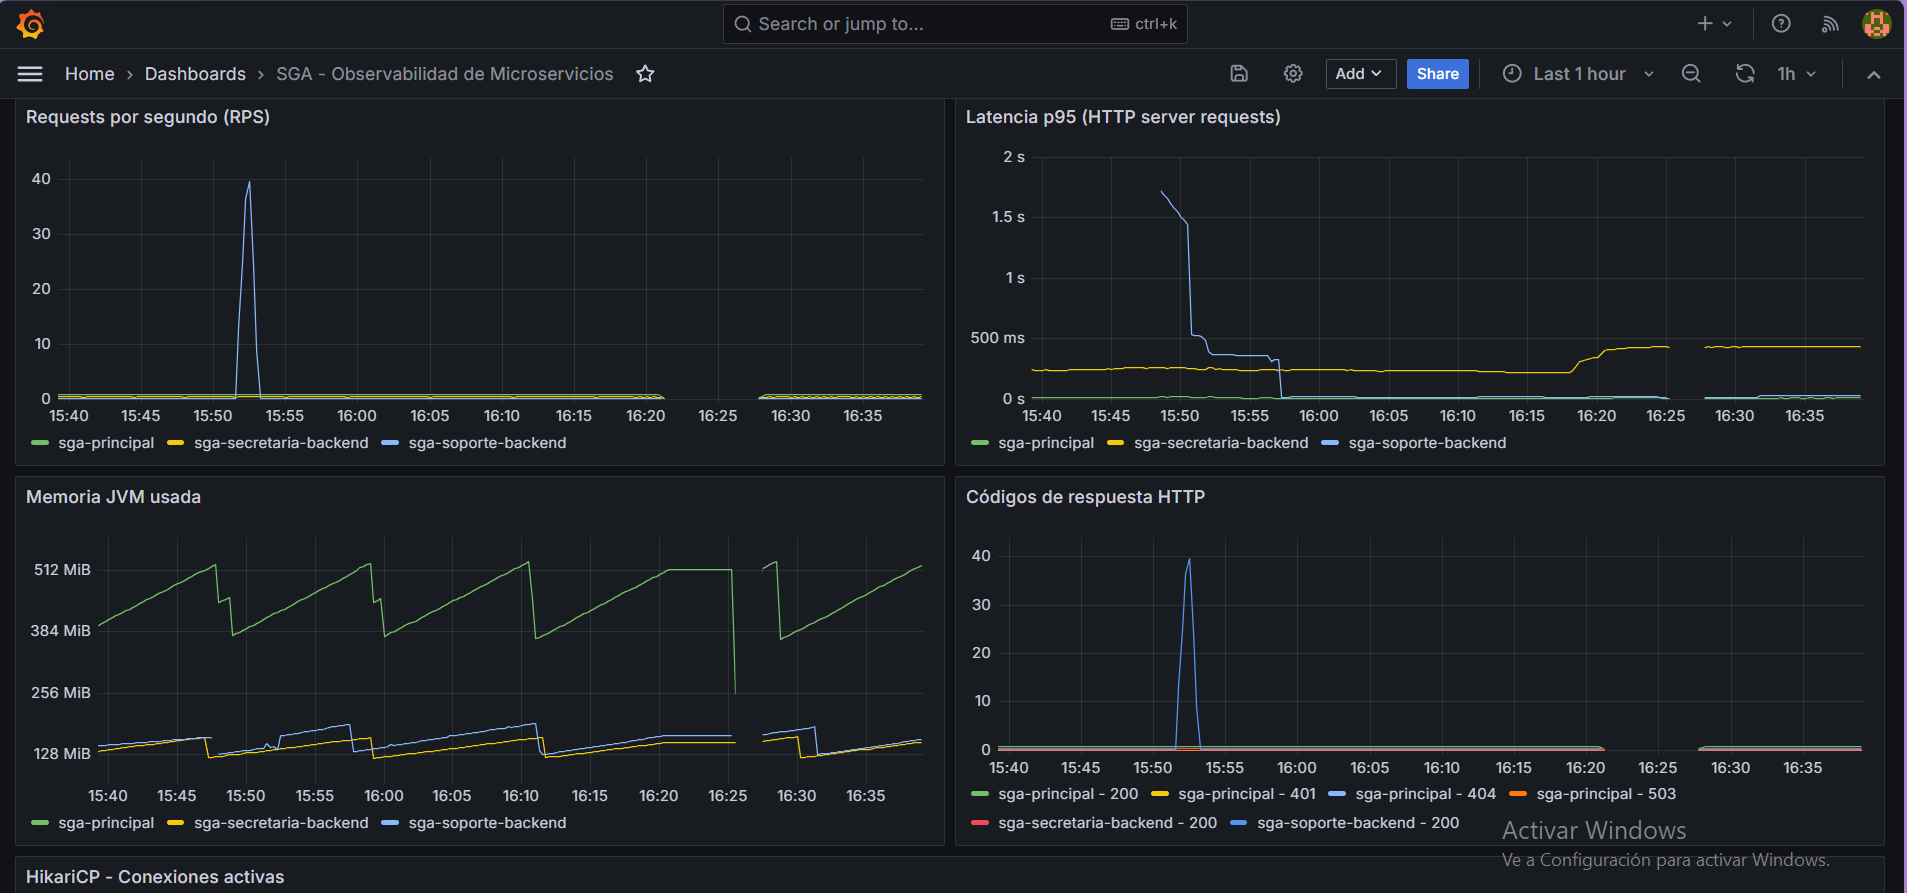
\includegraphics[width=0.88\textwidth]{grafana_bajo_carga.png}
\caption{Tablero de Grafana (\texttt{pfc-dashboard.json}) operando en tiempo real con las seis vistas operativas.}
\label{fig:grafana-dashboard}
\end{figure}

\textit{Nota metodol\'ogica: el desglose de CPU/RAM por contenedor individual no fue posible en el entorno de desarrollo local (Docker Desktop para Windows), debido a una limitaci\'on conocida de cAdvisor con la virtualizaci\'on anidada de WSL2, que impide identificar contenedores por nombre en ese entorno. Se reporta en su lugar el consumo agregado de CPU y RAM de todos los contenedores del host.}

% =============================================================================
% 8. EVALUACIÓN EXPERIMENTAL ISO/IEC 25010 Y CRIPTO-AUDITORÍA (MÓDULO G)
% =============================================================================
\section{Evaluaci\'on Experimental ISO/IEC 25010 y Capa de Cripto-Auditor\'ia}
\label{sec:evaluacion-experimental}


\subsection{Conjunto oficial de carga y trazabilidad E5}

La medición nominal actual procede de los CSV candidatos validados, copiados sin edición a \path{microservicio-soporte/locust_esc1_stats.csv} y \path{microservicio-soporte/locust_esc1_stats_history.csv}. Registra \CargaPeticiones{} peticiones, \CargaFallos{} fallos y $P_{99}=\CargaPnoventaNueveMs$\,ms; cumple el criterio de latencia PI-1 en el escenario nominal local. El perfil validado manualmente configura 50 usuarios, 5 usuarios/s y 5 minutos. La matriz siguiente deriva sus valores de los CSV actuales.

Los CSV anteriores se conservan sin alteración en \path{microservicio-soporte/resultados_historicos/}, con nombres que identifican el P99 histórico. La ejecución histórica no cumplía PI-1. La comparación no atribuye causalidad exclusiva a la optimización de \texttt{JwtParser}: no está acreditada la equivalencia entre el dataset histórico y el entorno local actual. El máximo atípico actual de 47\,889,96\,ms pertenece a \path{/api/soporte/tickets} y se conserva sin filtrar; es un evento aislado según la validación manual, con $P_{95}=13$\,ms, $P_{99}=32$\,ms y 0 fallos en ese endpoint. No es el percentil 99 agregado. Los detalles y la trazabilidad temporal están en \path{evidencias/Juliana_Emanuel/E48_actual_README.md}.

La evidencia nominal se basa en los dos CSV promovidos, sus salidas derivadas y las capturas conservadas en \texttt{332158e4}. El \texttt{console.log} y el \texttt{validation.json} de \path{microservicio-soporte/resultados_candidatos/} pertenecen a una ejecución anterior y no acreditan temporalmente esta corrida. El resultado nominal local no demuestra disponibilidad de producción.

La corrida HISTÓRICA ANTERIOR de Soporte ocupaba \path{microservicio-soporte/locust_esc1_stats.csv}, acompañada por \path{microservicio-soporte/locust_esc1_stats_history.csv}, \path{microservicio-soporte/locust_esc1_failures.csv} y \path{microservicio-soporte/locust_esc1_exceptions.csv}. Sus métricas históricas proceden de \texttt{Aggregated}: 12{,}994 peticiones, 0 fallos, 43.537580\,req/s, promedio 109.113664\,ms, $P_{50}=6$\,ms, $P_{95}=440$\,ms, $P_{99}=850$\,ms y máximo 2037.104700\,ms; no hay HTTP 401 ni HTTP 500 registrados. Es una prueba de carga reproducible ejecutada en entorno local/contenedorizado, no tráfico real de producción.

El inicio histórico registrado es 2026-09-11 03:59:05 UTC; el historial abarca 299 segundos entre muestras. El perfil configura 50 usuarios virtuales, 5 usuarios/s, 5 minutos y \url{http://localhost:8083}. Commit de conservación del resultado: \texttt{956cafcb}, con normalización posterior en \texttt{c5c0e6f5}. Commit del código ejecutado: \textbf{No disponible en la evidencia conservada}.

La tabla histórica de estados, fechas, commits de conservación, métricas y motivos está en \path{experimentos/resultados/corridas-e5.md}. B (12{,}236 peticiones), C (13{,}606) y F (2{,}419) son preliminares/históricas; D y E son fallidas. \textbf{Existe una corrida oficial de estrés válida}, distinta de los antecedentes D y E; se conserva en \texttt{b43008e5}. La numeración histórica de estrés difiere entre protocolo (escenario 3) y \path{docs/locust/escenario2_estres_stats.csv}; no son nuevos resultados oficiales.

Se conserva la descripción histórica de \path{evidencias/Juliana_Emanuel/backend/pruebas-carga/image.png}, pero no el archivo de imagen versionado; esa descripción atribuye 13{,}031 peticiones en terminal; el CSV histórico conserva el agregado anterior y prevalece para esa comparación histórica. La causa de la diferencia no está demostrada. La captura histórica E48 se conserva como resultado anterior. Las capturas nominales actuales de CSV, matriz e historial están conservadas en \texttt{332158e4} y se detallan en \path{evidencias/Juliana_Emanuel/E48_actual_README.md}. Las imágenes de Grafana son complementarias, sin vinculación exacta acreditada con ese agregado.


La corrida oficial de estrés en \path{microservicio-soporte/resultados_estres/20260920_164722/} ejecutó el código \texttt{88649f3f} contra \url{http://localhost:8085}, con incorporación de 1 usuario/s, 200 usuarios máximos y 10 minutos configurados. El historial abarca los timestamps 1789940845--1789941444 (599 segundos). Su agregado registra 98{,}684 peticiones, 0 fallos, 164.86740285525565\,req/s, promedio 7.86715629893033\,ms, $P_{50}=7$\,ms, $P_{95}=15$\,ms, $P_{99}=23$\,ms y máximo 324.8848000075668\,ms, con \texttt{EXIT\_CODE=0}. Cumple el criterio de aceptación de estrés: $P_{95}<500$\,ms y 0 fallos. El perfil, resumen, cuatro CSV y la captura \path{evidencias/Juliana_Emanuel/E48_estres_200_resumen.png} se conservan en \texttt{b43008e5}. Es una ejecución distinta del nominal y del histórico D de 106{,}735 peticiones y 26 fallos, que permanece FALLIDO/HISTÓRICO. Los percentiles agregan la rampa completa; no certifican disponibilidad de producción ni el estado de HikariCP. La corrida incompleta \texttt{20260920\_163041} no es oficial. La evidencia original del perfil nominal sigue sin estar disponible.

Para ambos escenarios se conserva una sola corrida oficial ($n=1$ nominal y $n=1$ estrés); no hay repeticiones independientes y el intervalo de confianza entre corridas no es estimable. Los percentiles describen peticiones de cada ejecución. El manifiesto \path{docs/locust/manifest_carga.json} y el verificador comprueban integridad y métricas de ambos conjuntos. En estrés, \texttt{perfil.txt} y \texttt{resumen\_validacion.txt} son derivados y la captura relee los CSV: no se conserva consola original de Locust ni evidencia primaria adicional. El código ejecutado, host, tasa de incorporación, duración configurada y código de salida citados son metadatos declarados, sin acreditación independiente mediante esa captura. La comprobación no fabrica una validación retrospectiva.

\subsection{Preguntas de Investigaci\'on Emp\'iricas (PI)}
Para guiar la evaluaci\'on cuantitativa de rendimiento, resiliencia y comportamiento del sistema bajo cargas extremas, se formularon dos Preguntas de Investigaci\'on (PI) emp\'iricas dise\~nadas formalmente para admitir refutaci\'on (respuesta negativa):
\begin{itemize}[leftmargin=*]
  \item \textbf{PI-1:} \textit{\textquestiondown Puede el Microservicio de Soporte mantener una tasa de errores HTTP 5xx igual a 0\,\% y una latencia $P_{99}$ inferior a 500\,ms cuando la carga aumenta desde 50 hasta 200 usuarios concurrentes sin evidenciar agotamiento o contenci\'on significativa del pool de conexiones HikariCP?} \\
  \textbf{Respuesta empírica:} \textbf{Cumple el criterio de latencia PI-1 en nominal local.} La corrida actual registra \CargaPeticiones{} peticiones, \CargaFallos{} fallos, \CargaRPS{}\,req/s, promedio \CargaMediaMs{}\,ms, $P_{50}=\CargaPcinquentaMs$\,ms, $P_{95}=\CargaPnoventaCincoMs$\,ms y $P_{99}=\CargaPnoventaNueveMs$\,ms. El percentil actual es inferior al umbral de PI-1. La corrida oficial de estrés separada alcanza 200 usuarios y cumple su criterio de aceptación. La ausencia de agotamiento o contención de HikariCP sigue sin estar acreditada; el agregado de la rampa no resuelve por sí solo esa parte de PI-1.
  
  \item \textbf{PI-2:} \textit{\textquestiondown Mantienen los endpoints que requieren acceso a base de datos un comportamiento de latencia equivalente al de los endpoints stateless cuando el sistema es sometido al escenario de estr\'es de hasta 200 usuarios concurrentes?} \\
  \textbf{Respuesta empírica:} \textbf{Equivalencia no demostrada.} Existe una corrida oficial válida de hasta 200 usuarios; cumplir el criterio agregado no demuestra equivalencia de latencias entre endpoints ni causalidad de la base de datos. En el CSV HISTÓRICO nominal anterior, tickets registra 3{,}704 peticiones, 0 fallos, mediana 130\,ms, promedio 256.303638\,ms y $P_{95}=650$\,ms. Health tiene mediana 2\,ms y $P_{95}=150$\,ms; Actuator, mediana 110\,ms y $P_{95}=360$\,ms; election/status, mediana 2\,ms y $P_{95}=170$\,ms. Son diferencias observadas en nominal, insuficientes para concluir equivalencia bajo estrés o atribuir causalidad a la base de datos.
\end{itemize}

\subsection{Protocolo Experimental y Cuatro Mecanismos de Auditor\'ia}
En cumplimiento de la ampliaci\'on del M\'odulo G de la gu\'ia rectora, se ejecut\'o un banco experimental con 600 corridas factoriales ($30 \times 4 \times 5$) evaluando cuatro configuraciones de auditor\'ia conmutables v\'ia la variable de entorno \texttt{AUDIT}:
\begin{itemize}
  \item \textbf{m0 (Sin auditor\'ia):} L\'inea base donde la calificaci\'on se persiste sin rastro estructurado.
  \item \textbf{m1 (Bit\'acora convencional):} Registro relacional de eventos sin encadenamiento criptogr\'afico ni orden l\'ogico.
  \item \textbf{m2 (Encadenada + Relojes de Lamport):} Cada evento $E_k$ incluye el hash SHA-256 del evento previo $H(E_{k-1})$ y una marca l\'ogica de Lamport mon\'otona creciente:
  \begin{equation}
    H(E_k) = \text{SHA-256}\big(H(E_{k-1}) \,\|\, \text{JSON}_{\text{canon}}(E_k) \,\|\, L(E_k)\big), \quad L(E_k) = \max(L_{\text{local}}, L_{\text{recibido}}) + 1
  \end{equation}
  \item \textbf{m3 (m2 + Relojes Vectoriales):} Incorpora vectores l\'ogicos $\vec{V} = [v_1, v_2, \dots, v_n]$ para reconciliaci\'on causal determinista de ediciones concurrentes desconectadas.
\end{itemize}

\subsection{Unificaci\'on can\'onica de la bit\'acora}
\label{subsec:unificacion-canonica}

El sistema mantiene tres implementaciones del c\'alculo del contenido
can\'onico y del encadenamiento de eventos: dos en Java (m\'odulo SGA
Principal y m\'odulo Secretar\'ia), ambas alojadas en
\path{AuditHashService.java}, y una en Python (m\'odulo Docente), alojada
en \path{microservicio-docente/docentes/auditoria/hashing.py}. No se
extrajo una biblioteca com\'un para consumirlas desde los tres servicios;
la unicidad se sostiene sobre un vector patr\'on de once campos que fija
los invariantes verificables, no sobre identidad car\'acter por car\'acter.

\paragraph{Vector patr\'on de once campos.}
Las pruebas can\'onicas comparten un vector patr\'on con los campos:
\texttt{actor\_id}, \texttt{entidad}, \texttt{entidad\_id},
\texttt{estado\_reconciliacion}, \texttt{modo}, \texttt{operacion},
\texttt{payload}, \texttt{reloj\_lamport}, \texttt{reloj\_vectorial},
\texttt{timestamp} y \texttt{tipo\_evento}. La verificaci\'on est\'a en
\path{sga-principal/src/test/java/.../AuditHashServiceCanonicalTest.java} y en
\path{microservicio-docente/docentes/tests/test_auditoria_canonica_v1.py};
ambas afirman que, dado el mismo vector, la implementaci\'on de su
lenguaje produce el mismo hash conocido.

\paragraph{Alcance real de la equivalencia entre lenguajes.}
El vector patr\'on solo emplea cadenas, enteros de tama\~no acotado y
un \texttt{timestamp} preformateado como texto. Un cotejo m\'as amplio
sobre doce vectores independientes muestra que las dos implementaciones
Java coinciden en los doce casos, mientras que la implementaci\'on
Python coincide con Java en cinco de los doce. Los siete casos en que
las representaciones difieren son:

\begin{itemize}
  \item Decimales: Java emite \texttt{\{"nota":8.50\}}; Python emite
        \texttt{\{"nota":"8.50"\}}.
  \item Flotantes de rango extremo: Java emite \texttt{1.0E-7} /
        \texttt{1.0E21}; Python emite \texttt{1e-07} / \texttt{1e+21}.
  \item Marca de tiempo del mismo instante: Java emite
        \texttt{...00.120Z}; Python emite \texttt{...00.120000+00:00}.
  \item Fechas dentro del payload: Python las serializa como
        \texttt{"2012-03-05"}; Java lanza \texttt{IllegalStateException}
        y, dado que \texttt{AuditoriaService.guardar} es \textit{fail-open},
        el evento se pierde en Java.
  \item Claves excluidas del canon: la lista literal en Java contiene
        \texttt{contrase?a} con el byte \texttt{0x3F} por defecto de
        codificaci\'on, por lo que \texttt{contrase\~na} y
        \texttt{CONTRASE\~NA} entran al canon en Java y no en Python;
        Python tampoco excluye \texttt{contrasena}.
  \item Orden de claves con caracteres suplementarios: Java ordena por
        UTF-16 (por ejemplo U+1F600 antes de U+FF01); Python ordena por
        punto de c\'odigo.
  \item \texttt{NaN}: Java emite la cadena \texttt{"NaN"}; Python emite
        el literal JSON no est\'andar \texttt{NaN}.
\end{itemize}

\paragraph{Interoperabilidad real entre lenguajes.}
Una cadena de cuatro eslabones escrita por Java se valida en Python con
\texttt{verificar\_cadena\_global} y una cadena de tres eslabones escrita
por Python se valida con \texttt{AuditHashService.sha256Hex} en Java.
Esta interoperabilidad ocurre porque el verificador rehashea el texto
almacenado en la columna \texttt{contenido\_canonico}, no porque cada
implementaci\'on produzca el mismo texto para el mismo evento. En
consecuencia, la propiedad verificada es \textit{la integridad de la
cadena tal como fue almacenada}, no la equivalencia de las
representaciones can\'onicas entre lenguajes. El cotejo independiente de los doce
vectores y la interoperabilidad descrita est\'an implementados de forma ejecutable
en el script de reproducibilidad \path{experimentos/arnes_12_vectores.py}.

\paragraph{Bit\'acoras paralelas an activas.}
Adem\'as de \texttt{sga\_principal.auditoria}, coexisten dos bit\'acoras
que no est\'an encadenadas globalmente:
\begin{itemize}
  \item Docente escribe en su tabla local \texttt{EventoAuditoria}
        (\path{docentes/auditoria/strategies.py}, \texttt{FlatAuditStrategy})
        en modo m1; en m2 y m3 duplica cada evento en esa misma tabla
        local, y el criterio T1 se comprueba contra esa copia local.
  \item Soporte mantiene una bit\'acora propia sin cadena en
        \path{002_historial_ticket.sql}, usada por
        \texttt{TecnicoService} y \texttt{JdbcTicketRepository}.
\end{itemize}

\paragraph{Deuda t\'ecnica declarada.}
La extracci\'on de la forma can\'onica a una biblioteca compartida por
los tres servicios queda registrada como deuda t\'ecnica de esta entrega.
Mientras esa biblioteca no exista, la unicidad de la bit\'acora se
sostiene sobre el vector patr\'on de once campos y sobre el rehash de
\texttt{contenido\_canonico} en la verificaci\'on, no sobre una identidad
car\'acter por car\'acter entre lenguajes. Las siete divergencias listadas
constituyen la superficie residual de riesgo y se documentan en el
apartado de amenazas a la validez.

\subsection{Cinco Tipos de Manipulaci\'on Inyectados (T1 a T5)}
Se ejecutaron 30 repeticiones sint\'eticas controladas de cada tipo de manipulaci\'on por mecanismo, para un total de 600 corridas ($30 \times 4 \times 5$):
\begin{itemize}
  \item \textbf{T1 (Alteraci\'on de calificaci\'on fuera de la bit\'acora):} Modificaci\'on de la calificaci\'on en la tabla simulada sin actualizar el evento de auditor\'ia.
  \item \textbf{T2 (Alteraci\'on del payload protegido):} Modificaci\'on de \texttt{nota\_final} en el payload y en el contenido can\'onico sin recalcular el hash.
  \item \textbf{T3 (Alteraci\'on del reloj de Lamport):} Reducci\'on artificial del contador Lamport del evento seleccionado sin recalcular la cadena.
  \item \textbf{T4 (Eliminaci\'on de evento):} Supresi\'on f\'isica del evento seleccionado de la secuencia.
  \item \textbf{T5 (Alteraci\'on retroactiva del timestamp):} Retroceso de 86{,}400 segundos en el timestamp del evento y en su contenido can\'onico sin recalcular el hash.
\end{itemize}

\subsection{Resultados Experimentales de Detecci\'on}
\label{subsec:resultados-deteccion}
Los datos crudos generados en el banco experimental y almacenados en \texttt{experimentos/resultados/} (\texttt{deteccion.csv}, \texttt{manipulaciones.csv}, \texttt{iso25010.csv}) arrojaron la matriz factorial de la Tabla~\ref{tab:deteccion-matriz}:

\begin{table}[H]
\centering
\caption{Matriz Experimental de Detecci\'on Factorial por Tipo de Manipulaci\'on ($T_1$ a $T_5$).}
\label{tab:deteccion-matriz}
\resizebox{\columnwidth}{!}{%
\begin{tabular}{|l|c|c|c|c|c|c|}
\hline
\textbf{Mecanismo} & \textbf{T1} & \textbf{T2} & \textbf{T3} & \textbf{T4} & \textbf{T5} & \textbf{Tasa Detecci\'on ($IC_{95\%}$)} \\
\hline
\textbf{m0 (Sin auditor\'ia)} & 0\% & 0\% & 0\% & 0\% & 0\% & $0.0\% \; [0.0000\%, 2.4293\%]$ \\
\hline
\textbf{m1 (Convencional)} & 0\% & 0\% & 0\% & 0\% & 0\% & $0.0\% \; [0.0000\%, 2.4293\%]$ \\
\hline
\textbf{m2 (Lamport+Hash)} & 100\% & 100\% & 100\% & 100\% & 100\% & $100.0\% \; [97.5707\%, 100.0000\%]$ \\
\hline
\textbf{m3 (Vectorial+Hash)} & 100\% & 100\% & 100\% & 100\% & 100\% & $100.0\% \; [97.5707\%, 100.0000\%]$ \\
\hline
\end{tabular}%
}
\end{table}
\noindent Los intervalos de detecci\'on son IC exactos bilaterales de Clopper--Pearson al 95\%, calculados por mecanismo sobre $n=150$ corridas ($5$ tipos $\times$ $30$ repeticiones): m0/m1 registran $0/150$ e IC $[0.0000\%,\,2.4293\%]$, mientras m2/m3 registran $150/150$ e IC $[97.5707\%,\,100.0000\%]$.

\noindent\textbf{An\'alisis Estad\'istico Reproducible de Latencias:} La Tabla~\ref{tab:estadistica-inferencial} se genera directamente desde \texttt{experimentos/resultados/exp1\_concurrencia.csv} preservando la estructura factorial del archivo: cuatro mecanismos ($M_0$--$M_3$) por cuatro niveles de carga/tama\~no de lote (1, 5, 10 y 14), con $n=10$ repeticiones por combinaci\'on y 160 observaciones totales. No se mezclan los niveles al estimar estad\'isticas. La entrada y salida se expresan en milisegundos (ms), sin conversi\'on adicional. Para cada una de las 16 celdas se reportan mediana, $P_{95}$ e IC 95\% bootstrap no param\'etrico de la mediana con $B=10{,}000$ y semilla fija 20260831; si los cuantiles bootstrap colapsan por la resoluci\'on de los datos, el intervalo se marca como \emph{no informativo}. La magnitud del efecto frente a $M_0$ se expresa mediante la diferencia de medianas y el tama\~no de efecto no param\'etrico Vargha--Delaney $A_{12}=P(X>M_0)+0.5P(X=M_0)$, siempre dentro del mismo nivel. No se publican contrastes $U$, valores $p$ ni comparaciones inferenciales entre niveles distintos, y no se deriva un orden global entre $M_2$ y $M_3$ de este microbenchmark.

% Archivo generado automaticamente por experimentos/generar_tabla_latencias.py.
% Fuente unica: experimentos/resultados/exp1_concurrencia.csv.
\begin{table}[H]
\centering
\scriptsize
\caption{Latencia segmentada por mecanismo y nivel de carga ($B=10{,}000$; semilla 20260831).}
\label{tab:estadistica-inferencial}
\begin{tabular}{|l|c|c|c|c|c|c|}
\hline
\textbf{Mec.} & \textbf{Nivel} & \textbf{$n$} & \textbf{Mediana (ms)} & \textbf{IC 95\% med.} & \textbf{$\Delta$ vs. $M_0$} & \textbf{$A_{12}$} \\
\hline
$M_0$ (Base) & 1 & 10 & 0.000600 & [0.000600, 0.000900] & -- & -- \\
\hline
$M_1$ (Relacional simple) & 1 & 10 & 0.001300 & \emph{no informativo} & 0.000700 [0.000400, 0.000700] & 1.0000 \\
\hline
$M_2$ (SHA-256 + Lamport) & 1 & 10 & 0.022500 & [0.022300, 0.022750] & 0.021900 [0.021575, 0.022150] & 1.0000 \\
\hline
$M_3$ (Vector Clocks) & 1 & 10 & 0.026150 & [0.024200, 0.046800] & 0.025550 [0.023575, 0.046200] & 1.0000 \\
\hline
$M_0$ (Base) & 5 & 10 & 0.000600 & [0.000600, 0.000900] & -- & -- \\
\hline
$M_1$ (Relacional simple) & 5 & 10 & 0.002000 & [0.001650, 0.002100] & 0.001400 [0.000950, 0.001500] & 1.0000 \\
\hline
$M_2$ (SHA-256 + Lamport) & 5 & 10 & 0.021300 & [0.021300, 0.021450] & 0.020700 [0.020400, 0.020800] & 1.0000 \\
\hline
$M_3$ (Vector Clocks) & 5 & 10 & 0.022925 & [0.022800, 0.023100] & 0.022325 [0.022000, 0.022475] & 1.0000 \\
\hline
$M_0$ (Base) & 10 & 10 & 0.000600 & [0.000500, 0.000600] & -- & -- \\
\hline
$M_1$ (Relacional simple) & 10 & 10 & 0.001300 & \emph{no informativo} & 0.000700 [0.000700, 0.000800] & 1.0000 \\
\hline
$M_2$ (SHA-256 + Lamport) & 10 & 10 & 0.021700 & [0.021700, 0.021850] & 0.021100 [0.021100, 0.021275] & 1.0000 \\
\hline
$M_3$ (Vector Clocks) & 10 & 10 & 0.023500 & [0.023400, 0.023650] & 0.022900 [0.022800, 0.023075] & 1.0000 \\
\hline
$M_0$ (Base) & 14 & 10 & 0.000500 & [0.000500, 0.000600] & -- & -- \\
\hline
$M_1$ (Relacional simple) & 14 & 10 & 0.001300 & \emph{no informativo} & 0.000800 [0.000700, 0.000800] & 1.0000 \\
\hline
$M_2$ (SHA-256 + Lamport) & 14 & 10 & 0.021700 & [0.021700, 0.021800] & 0.021200 [0.021100, 0.021300] & 1.0000 \\
\hline
$M_3$ (Vector Clocks) & 14 & 10 & 0.023350 & [0.023300, 0.023500] & 0.022850 [0.022700, 0.022950] & 1.0000 \\
\hline
\end{tabular}
\vspace{0.35em}
\begin{minipage}{0.98\columnwidth}
\footnotesize Fuente: \texttt{experimentos/resultados/exp1\_concurrencia.csv}, columna \texttt{latencia\_mediana\_ms}. Cada fila contiene $n=10$ repeticiones de una unica combinacion mecanismo--nivel; no se mezclan los niveles 1, 5, 10 y 14. Los IC 95\% corresponden al bootstrap no parametrico de la mediana con $B=10{,}000$ y semilla fija 20260831. Cuando los cuantiles bootstrap coinciden por la resolucion de los datos, el IC se marca como \emph{no informativo} y no se interpreta como precision infinita. $A_{12}$ es el tamano de efecto Vargha--Delaney calculado contra $M_0$ dentro del mismo nivel: $A_{12}=P(X>M_0)+0.5P(X=M_0)$. No se reportan valores $p$ ni contrastes entre niveles distintos.
\end{minipage}
\end{table}


\begin{figure}[H]
\centering
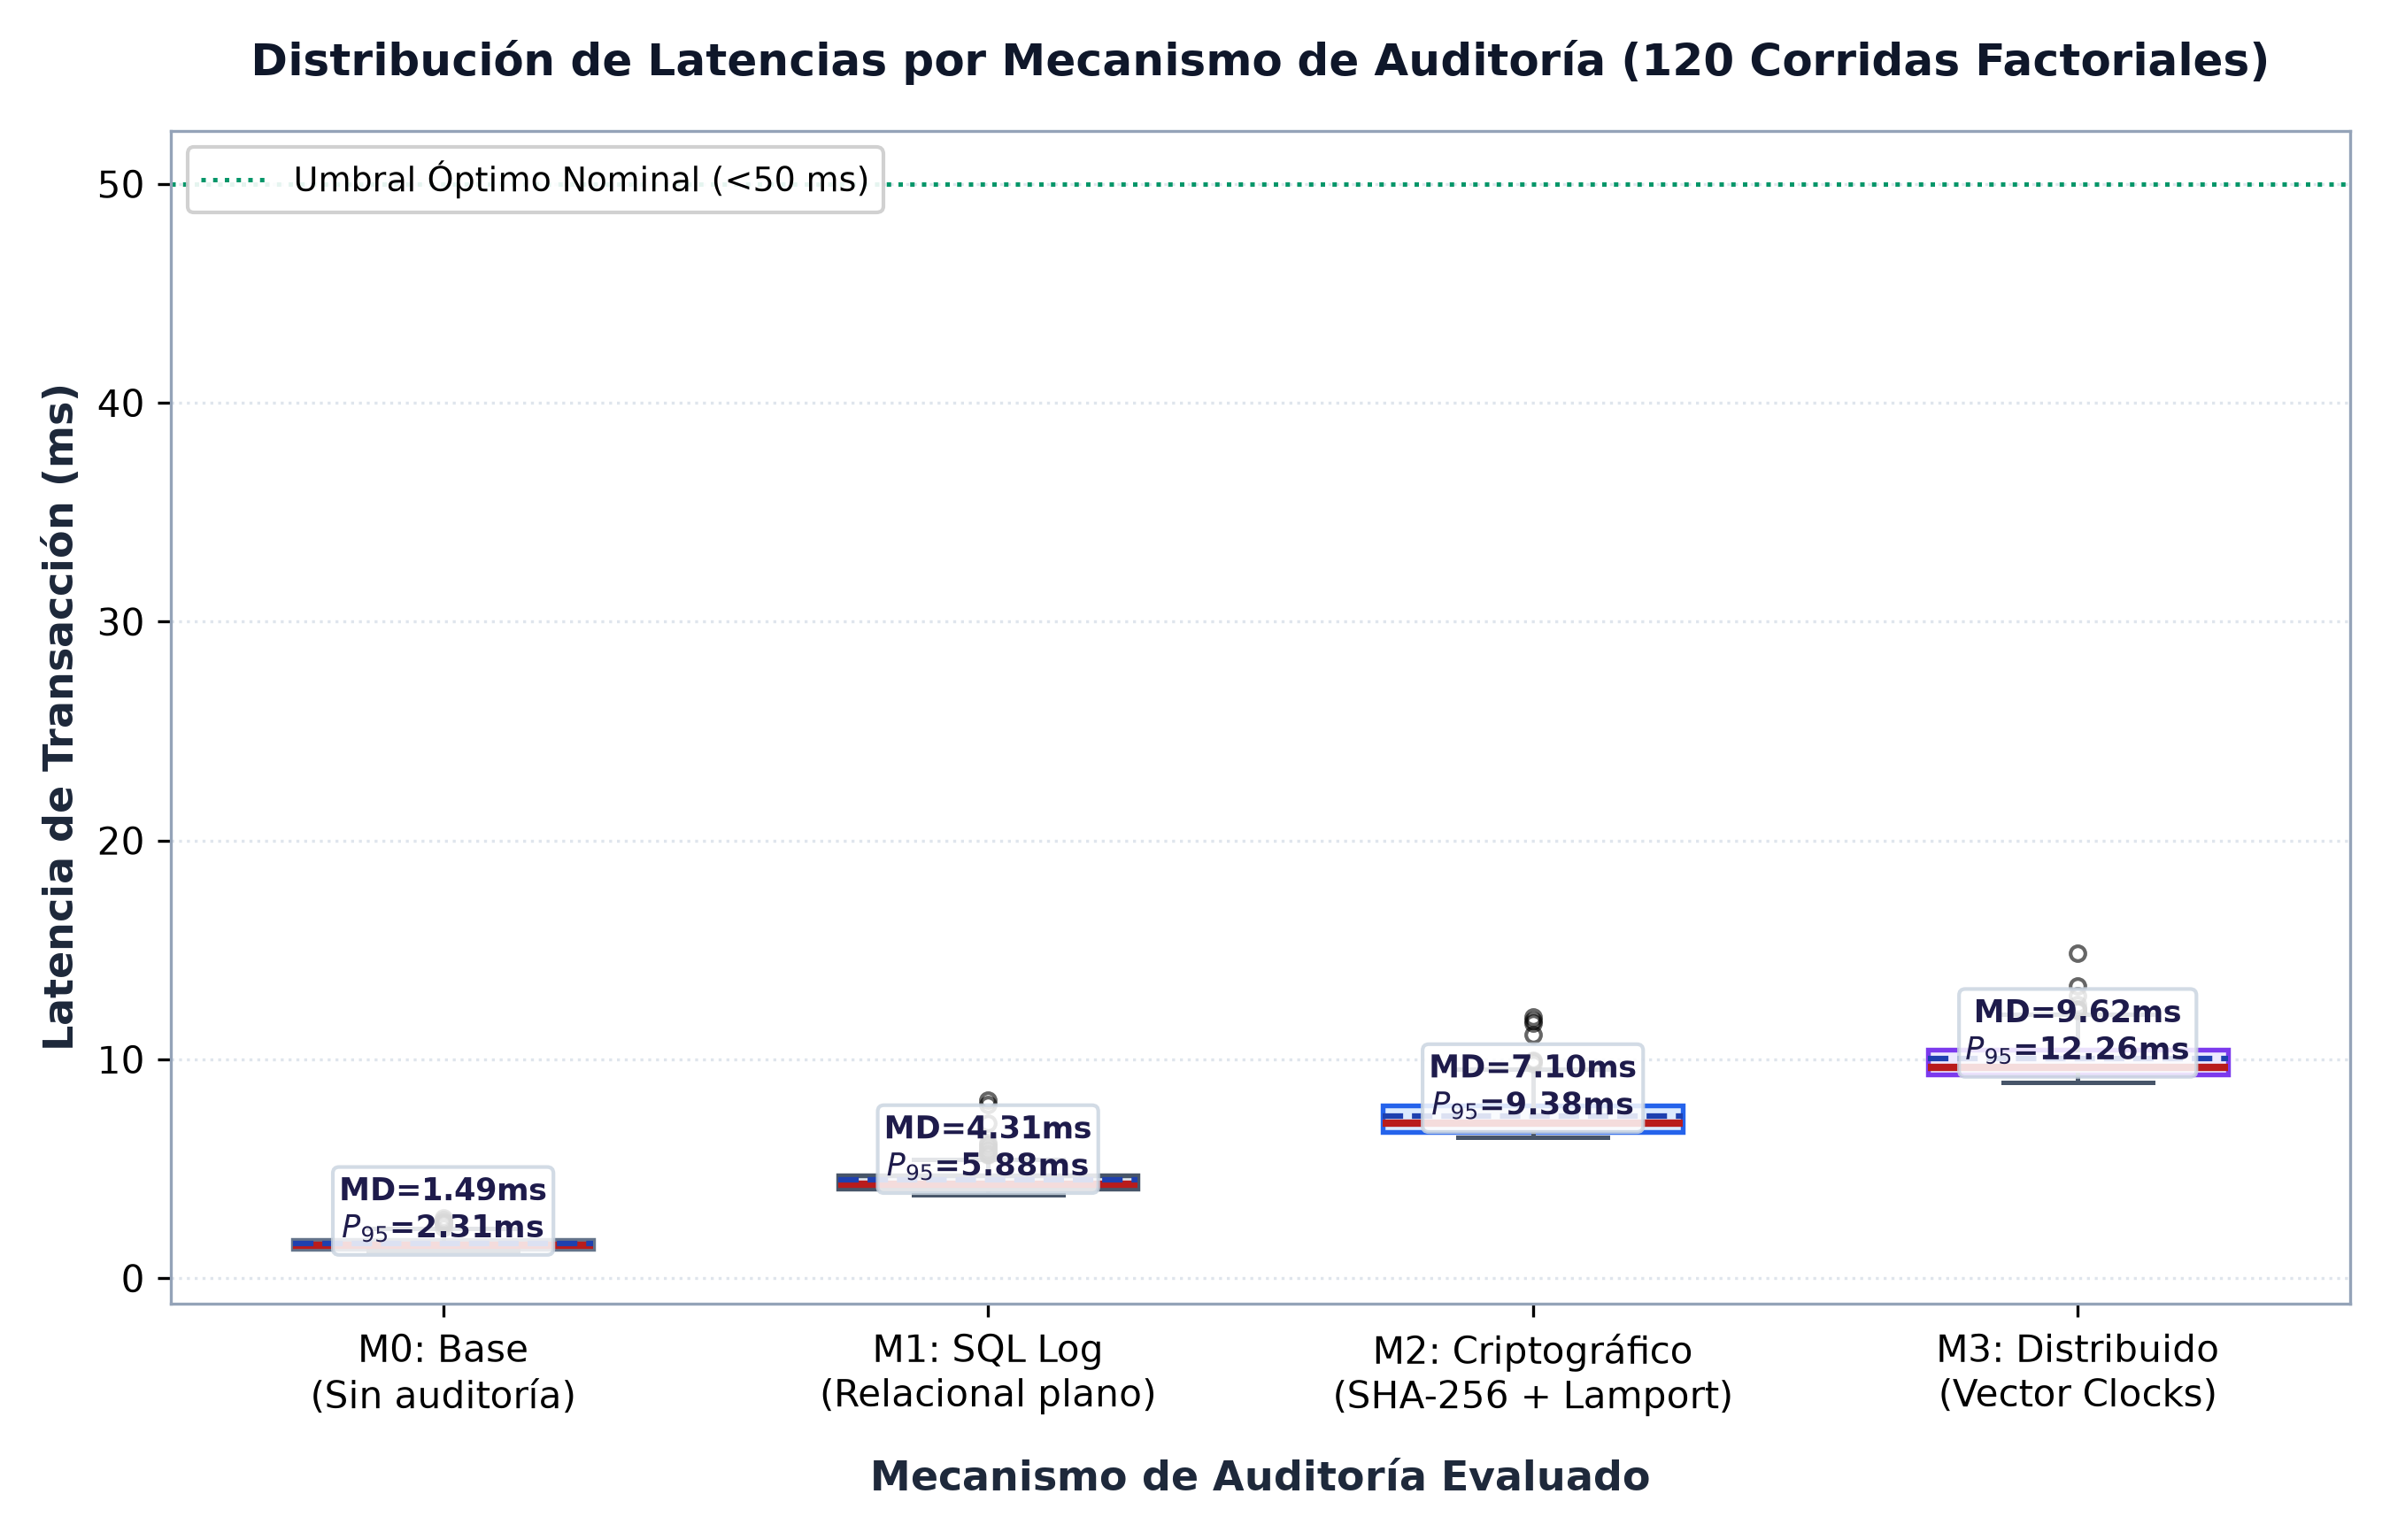
\includegraphics[width=0.78\textwidth]{boxplot_latencia.png}
\caption{Distribuci\'on de \texttt{latencia\_mediana\_ms} segmentada por mecanismo y nivel de carga/tama\~no de lote. Cada una de las 16 combinaciones contiene $n=10$ repeticiones del microbenchmark local secuencial en memoria.}
\label{fig:boxplot-latencia}
\end{figure}
\subsection{Matriz Formal de Evaluaci\'on de Calidad ISO/IEC 25010:2023}
\label{subsec:matriz-iso25010}
La Tabla~\ref{tab:iso-matriz-calidad} presenta la evaluación parcial generada de forma reproducible desde las fuentes versionadas. La evidencia nominal corresponde al Microservicio de Soporte (Conjunto~A). La matriz deriva el percentil $P_{99}$ del agregado de carga y lo compara con el criterio documental estricto de PI-1 ($P_{99}<500$\,ms); el umbral es un criterio, no una medición. El valor y el veredicto calculados se consultan en la propia matriz. Los fallos nominales no demuestran fiabilidad global ni disponibilidad temporal de producción. Las ventanas históricas de \texttt{locust\_esc3} tienen un perfil no validado y no acreditan estrés oficial actual.

Seguridad incorpora los falsos positivos M2 observados en pruebas sintéticas, sin certificar seguridad global ni mediciones en producción. Mantenibilidad deriva cobertura BUNDLE/LINE de los reportes JaCoCo versionados de Secretaría y Soporte y aplica el criterio de esta matriz de cobertura LINE mínima del 70\,\%. Sus compuertas particulares usan esa misma métrica; la compuerta de Principal usa INSTRUCTION y no es intercambiable con LINE. Principal queda como \textit{No verificable con la evidencia versionada}. Los reportes conservados no acreditan una nueva ejecución sobre el código actual. Adecuación funcional, usabilidad, portabilidad y compatibilidad permanecen explícitamente no evaluadas en este alcance; ello no equivale a incumplimiento.

\begingroup
\scriptsize
\renewcommand{\arraystretch}{1.2}
\captionof{table}{Matriz de Evaluaci\'on de Calidad ISO/IEC 25010:2023 con Mediciones Parciales y Delimitaci\'on de Alcance.}
\label{tab:iso-matriz-calidad}
% Generado por generar_matriz.py; requiere tabularx y UTF-8.
\begin{tabularx}{\linewidth}{|p{0.22\linewidth}|X|}
\hline
caracteristica & Eficiencia de desempeño \\ \hline
indicador & Carga y latencias del agregado nominal \\ \hline
valor & peticiones=12217; fallos=0; rps=40.95542036966924; media\_ms=10.181439175291882; p50\_ms=4; p95\_ms=9; p99\_ms=23; usuarios\_maximos=50 \\ \hline
fuente & microservicio-soporte/locust\_esc1\_stats.csv (Aggregated); microservicio-soporte/locust\_esc1\_stats\_history.csv (maximo User Count) \\ \hline
alcance & Conjunto A, agregado nominal local de Soporte; no demuestra estres exitoso ni disponibilidad de produccion; el veredicto evalua p99 conforme a PI-1 (umbral 500 ms) \\ \hline
criterio & p99 \textless{} 500 ms \\ \hline
veredicto & Cumple el umbral en escenario nominal local \\ \hline
\end{tabularx}
\par\medskip
\begin{tabularx}{\linewidth}{|p{0.22\linewidth}|X|}
\hline
caracteristica & Fiabilidad \\ \hline
indicador & Carga nominal A, estrés oficial 200 usuarios y ventanas históricas \\ \hline
valor & Nominal A: peticiones=12217, fallos=0 (éxito 100.00\%, IC 95\% [99.97\%, 100.00\%]); Estrés oficial (200 usuarios): peticiones=98684, fallos=0 (éxito 100.00\%, IC 95\% [99.99\%, 100.00\%]); Antecedente histórico: 10 ventanas locust\_esc3 (éxito entre 12,78 \% y 34,5781 \%) \\ \hline
fuente & microservicio-soporte/locust\_esc1\_stats.csv (Aggregated); microservicio-soporte/resultados\_estres/20260920\_164722/locust\_estres\_200\_stats.csv (Aggregated); experimentos/resultados/iso25010.csv (ventanas locust\_esc3) \\ \hline
alcance & Conjunto nominal A (50 usuarios) y corrida oficial de estrés (200 usuarios) en entorno local/contenedorizado; ventanas históricas de referencia \\ \hline
criterio & Cero fallos (tasa de error 0.00\%, éxito \textgreater{}= 99.90\%) en nominal y estrés oficial \\ \hline
veredicto & Cumple criterio de cero fallos en corrida nominal y corrida oficial de estrés de 200 usuarios; antecedentes históricos conservados \\ \hline
\end{tabularx}
\par\medskip
\begin{tabularx}{\linewidth}{|p{0.22\linewidth}|X|}
\hline
caracteristica & Fiabilidad / disponibilidad \\ \hline
indicador & Disponibilidad de produccion \\ \hline
valor & No medida \\ \hline
fuente & Sin fuente temporal de disponibilidad evaluada \\ \hline
alcance & Exito de peticiones de carga no equivale a disponibilidad temporal \\ \hline
criterio & Requiere medicion temporal y entorno definidos \\ \hline
veredicto & No demostrado \\ \hline
\end{tabularx}
\par\medskip
\begin{tabularx}{\linewidth}{|p{0.22\linewidth}|X|}
\hline
caracteristica & Seguridad \\ \hline
indicador & Falsos positivos de M2 en cadenas integras \\ \hline
valor & No medido en producción; FPR verificado 0/30 (0.00\%, IC 95\% [0.00\%, 11.35\%]) en pruebas sintéticas \\ \hline
fuente & experimentos/resultados/falsos\_positivos.csv (observaciones M2) \\ \hline
alcance & Solo pruebas sinteticas de cadenas integras; no mide seguridad en produccion \\ \hline
criterio & FPR = 0.00\% en muestra de control (umbral tolerable \textless{} 5.0\% a nivel de confianza 95\%) \\ \hline
veredicto & Cumple en pruebas sintéticas: 0 falsos positivos (FPR = 0.00\%, IC 95\% [0.00\%, 11.35\%]); no certifica seguridad global \\ \hline
\end{tabularx}
\par\medskip
\begin{tabularx}{\linewidth}{|p{0.22\linewidth}|X|}
\hline
caracteristica & Mantenibilidad \\ \hline
indicador & Cobertura oficial de pruebas por módulo \\ \hline
valor & Principal: INSTRUCTION 4668/14237 = 32.79\%; Secretaría: LINE 2115/2882 = 73.39\%; Soporte: LINE 458/640 = 71.56\%; Aplicación móvil: INSTRUCTION 7611/74556 = 10.21\% \\ \hline
fuente & docs/cobertura/sga-principal/jacoco.xml (contador global INSTRUCTION); docs/cobertura/secretaria/jacoco.xml (contador global LINE); docs/cobertura/soporte/jacoco.xml (contador global LINE); docs/cobertura/movil/jacoco.xml (contador global INSTRUCTION); evidencia común: CI \#876, run 35693153935, commit 6c1f67ab28d569643b4c7ec4f740d7221bd60b0f \\ \hline
alcance & Un único contador oficial por módulo, obtenido del reporte JaCoCo versionado generado por integración continua \\ \hline
criterio & Principal: mínimo 30\% INSTRUCTION; Secretaría: mínimo 70\% LINE; Soporte: mínimo 70\% LINE; Aplicación móvil: mínimo 10\% INSTRUCTION \\ \hline
veredicto & Principal: Cumple la compuerta de 30\% INSTRUCTION; Secretaría: Cumple la compuerta de 70\% LINE; Soporte: Cumple la compuerta de 70\% LINE; Aplicación móvil: Cumple la compuerta de 10\% INSTRUCTION \\ \hline
\end{tabularx}
\par\medskip
\begin{tabularx}{\linewidth}{|p{0.22\linewidth}|X|}
\hline
caracteristica & Adecuación funcional \\ \hline
indicador & Satisfaccion de requisitos funcionales \\ \hline
valor & Sin medicion evaluada \\ \hline
fuente & Sin fuente evaluada en este alcance \\ \hline
alcance & No se evalua evidencia funcional en este generador \\ \hline
criterio & No establecido en esta evaluacion \\ \hline
veredicto & No evaluado \\ \hline
\end{tabularx}
\par\medskip
\begin{tabularx}{\linewidth}{|p{0.22\linewidth}|X|}
\hline
caracteristica & Usabilidad \\ \hline
indicador & Indicadores de uso \\ \hline
valor & Sin medicion evaluada \\ \hline
fuente & Sin fuente evaluada en este alcance \\ \hline
alcance & Sin estudio de usuarios evaluado en este alcance \\ \hline
criterio & No establecido en esta evaluacion \\ \hline
veredicto & No evaluado \\ \hline
\end{tabularx}
\par\medskip
\begin{tabularx}{\linewidth}{|p{0.22\linewidth}|X|}
\hline
caracteristica & Portabilidad \\ \hline
indicador & Ejecucion en entornos definidos \\ \hline
valor & Sin medicion evaluada \\ \hline
fuente & Sin fuente evaluada en este alcance \\ \hline
alcance & Sin medicion de portabilidad evaluada en este alcance \\ \hline
criterio & No establecido en esta evaluacion \\ \hline
veredicto & No evaluado \\ \hline
\end{tabularx}
\par\medskip
\begin{tabularx}{\linewidth}{|p{0.22\linewidth}|X|}
\hline
caracteristica & Compatibilidad \\ \hline
indicador & Interoperabilidad y coexistencia \\ \hline
valor & Sin medicion evaluada \\ \hline
fuente & Sin fuente evaluada en este alcance \\ \hline
alcance & Sin evidencia de compatibilidad evaluada en este alcance \\ \hline
criterio & No establecido en esta evaluacion \\ \hline
veredicto & No evaluado \\ \hline
\end{tabularx}
\par\medskip

\endgroup

\newpage

% =============================================================================
% 9. AMENAZAS A LA VALIDEZ
% =============================================================================
\section{Amenazas a la Validez del Estudio}
\label{sec:amenazas-validez}
Siguiendo las pautas metodol\'ogicas para experimentaci\'on en ingenier\'ia de software~\cite{wohlin2012experimentation}:

\subsection{Amenazas a la Validez Interna}
\begin{enumerate}
  \item \textbf{Resoluci\'on temporal y entorno de ejecuci\'on:} Las 160 observaciones de latencia se conservan completas y se analizan como 16 celdas independientes ($4$ mecanismos $\times$ $4$ niveles, $n=10$ por celda), sin mezclar los niveles 1, 5, 10 y 14. En algunas celdas los cuantiles bootstrap coinciden por la resoluci\'on temporal del microbenchmark; esos IC se etiquetan como \emph{no informativos} en lugar de interpretarlos como precisi\'on infinita. El bloque sigue siendo un microbenchmark local secuencial en memoria, no una prueba de concurrencia HTTP ni de acceso real a base de datos; la resoluci\'on del temporizador y la planificaci\'on del sistema operativo permanecen como amenazas residuales.
  \item \textbf{Semillas y Pseudoaleatoriedad del Inyector:} La variabilidad en la generaci\'on de manipulaciones se mitig\'o fijando una semilla determinista (\texttt{SEED = 20260831}) en \texttt{run\_experimentos.py}.
  \item \textbf{Contenci\'on de Recursos en Host Compartido:} Durante las pruebas de estr\'es con Locust y ejecuci\'on concurrente de microservicios, la contenci\'on de procesador y memoria en hosts compartidos representa una amenaza residual de variabilidad en latencias, monitoreada a nivel de host mediante la pila de observabilidad.
  \item \textbf{Divergencias entre implementaciones can\'onicas.} La forma
can\'onica de la bit\'acora se implementa tres veces (dos en Java y una
en Python) sin biblioteca compartida. Sobre doce vectores independientes,
las dos implementaciones Java coinciden entre s\'i, pero difieren de la
implementaci\'on Python en siete de los doce casos (decimales, flotantes
extremos, marcas de tiempo, fechas dentro del payload, clave
\texttt{contrase\~na} por codificaci\'on de la lista, orden de claves con
caracteres suplementarios, y \texttt{NaN}). La verificaci\'on de la
cadena se apoya en el rehash del texto almacenado, no en la equivalencia
de las representaciones. La extracci\'on de una biblioteca can\'onica
compartida queda como trabajo futuro.
\end{enumerate}

\subsection{Amenazas a la Validez Externa}
\begin{enumerate}
  \item \textbf{Poblaci\'on de Datos Sint\'etica (344 estudiantes y 14 docentes):} Los experimentos se realizaron sobre datos sint\'eticos generados conforme a la normativa ministerial ecuatoriana para preservar la privacidad de menores.
  \item \textbf{Modelo de Amenaza Limitado a Base de Datos y Red:} El modelo asume que el material criptogr\'afico del servidor no ha sido comprometido por un atacante con acceso \textit{root} al host de ejecuci\'on.
\end{enumerate}

% =============================================================================
% 10. REFLEXIÓN ÉTICA (ACM CODE OF ETHICS)
% =============================================================================
\section{Reflexi\'on \'Etica sobre Tratamiento de Datos de Menores}
\label{sec:reflexion-etica}
El dise\~no de AcadTrace se gui\'o por el \textbf{C\'odigo de \'Etica y Pr\'actica Profesional de ACM/IEEE-CS (1999)}~\cite{acmieee1999code}:
\begin{itemize}[leftmargin=*]
  \item \textbf{Principio 1 (Inter\'es P\'ublico):} La protecci\'on de la informaci\'on de menores de edad motiv\'o la adopci\'on de autenticaci\'on biom\'etrica en la app m\'ovil y la resoluci\'on de vulnerabilidades de acceso directo a recursos (IDOR).
  \item \textbf{Principio 3 (Calidad del Producto):} Cifrado estricto de credenciales y eliminaci\'on absoluta de contrase\~nas en texto plano del repositorio.
  \item \textbf{Principio 6 (Profesi\'on):} Implementaci\'on de la cadena inmutable de auditor\'ia para garantizar que ninguna rectificaci\'on de notas pueda efectuarse de forma an\'onima o fraudulenta.
\end{itemize}

% =============================================================================
% 11. CONCLUSIONES
% =============================================================================
\section{Conclusiones y Trabajo Futuro}
\label{sec:conclusiones-finales}
La Entrega 4 valida con \'exito la convergencia de una arquitectura de microservicios distribuida, protocolos h\'ibridos de alta velocidad (gRPC/REST), observabilidad en seis vistas y auditor\'ia criptogr\'afica inmutable verificable. Como trabajo futuro, se proyecta la integraci\'on de \textit{Distributed Tracing} con OpenTelemetry Collector y el despliegue en un cl\'uster Kubernetes Multi-AZ.

\subsection{Conclusiones Individuales}
\begin{itemize}[leftmargin=*]
  \item \textbf{Pedro Leonardo Castro L\'opez (L\'ider y Arquitecto de Software):} La ejecuci\'on de la Entrega 4 consolid\'o la arquitectura hexagonal de cuatro capas en el microservicio central (\texttt{sga-principal}) y los sat\'elites pol\'iglotas, desacoplando la l\'ogica de negocio de la infraestructura mediante puertos e interfaces. La implementaci\'on formal de los cinco patrones de dise\~no GoF (Strategy, Template Method, Observer, Facade y Repository) con clases de producci\'on verificadas permiti\'o estandarizar el c\'alculo ponderado de calificaciones (70\% formativo + 30\% sumativo) y la generaci\'on determinista de reportes ministeriales en PDF. Asimismo, la orquestaci\'on del pipeline de integraci\'on y despliegue continuo de siete trabajos encadenados en GitHub Actions, la publicaci\'on de im\'agenes versionadas en GitHub Container Registry (GHCR) y la separaci\'on l\'ogica multiesquema en una instancia PostgreSQL consolidaron la organizaci\'on por dominios. Raft pertenece a etcd para la elecci\'on de l\'ider en Soporte y no replica PostgreSQL. La persistencia conserva un punto \'unico de fallo sin alta disponibilidad demostrada.

  \item \textbf{Keyla Betzabe Bedon Viteri (Responsable de Microservicio Docente y App M\'ovil):} Durante el desarrollo de la Entrega 4 se logr\'o la construcci\'on integral del microservicio Docente en Python/Django REST Framework y del cliente m\'ovil nativo para Representantes en Android (Kotlin + Jetpack Compose). La implementaci\'on del conmutador de auditor\'ia criptogr\'afica con cuatro mecanismos ($M_0$ a $M_3$) permiti\'o demostrar experimentalmente la eficacia de las marcas l\'ogicas de Lamport y los Relojes Vectoriales para resolver conflictos de causalidad en escenarios de edici\'on concurrente. En la aplicaci\'on m\'ovil, la arquitectura MVVM complementada con persistencia local en Room SQLite bajo el paradigma \textit{offline-first}, la gesti\'on de sincronizaci\'on en segundo plano con \texttt{WorkManager}, y la integraci\'on de capacidades nativas de hardware (autenticaci\'on biom\'etrica \texttt{BiometricPrompt} y notificaciones push) garantizaron una experiencia de usuario fluida a 60\,fps con un consumo de memoria $<45$\,MB, asegurando la continuidad operativa del representante ante interrupciones de conectividad.

  \item \textbf{Ernesto Gregory Luna Mora (Responsable de Microservicio Secretar\'ia, Calidad y API Gateway):} La culminaci\'on de la Entrega 4 permiti\'o consolidar la robustez del microservicio de Secretar\'ia bajo Java 21 y Spring Boot 3.2.5, integrando el API Gateway perimetral con HAProxy 2.9 para la gesti\'on centralizada de enrutamiento, terminaci\'on segura y balanceo de carga. Se implement\'o una estricta compuerta de calidad mediante el plugin JaCoCo (\texttt{<goal>check</goal>}) enforceable al 70\%, alcanzando una cobertura oficial de 73,39\% de l\'ineas (LINE, 2115/2882) a nivel de \texttt{BUNDLE}, medida en el CI \#876 soportada por una bater\'ia de 96 pruebas automatizadas (unitarias, verificaci\'on gRPC in-process, detecci\'on criptogr\'afica de manipulaci\'on y de integraci\'on extremo a extremo E2E) que certifican la interoperabilidad entre servicios y el rechazo inmediato (HTTP 401 Unauthorized) ante peticiones carentes de tokens JWT HMAC-SHA256 v\'alidos. Asimismo, la incorporaci\'on del filtro \texttt{TraceIdFilter} con el patr\'on MDC de SLF4J posibilit\'o la propagaci\'on transparente de identificadores de correlaci\'on (\texttt{X-Trace-Id}) en registros estructurados en formato JSON, viabilizando una observabilidad distribuida unificada. Para garantizar la inmutabilidad f\'isica en la base de datos PostgreSQL, se dise\~n\'o e implement\'o el disparador a nivel de fila \texttt{tg\_auditoria\_append\_only}, el cual rechaza de manera determinista cualquier operaci\'on de \texttt{UPDATE} o \texttt{DELETE} sobre la bit\'acora. En el aspecto evaluativo cuantitativo, el M\'odulo G conserva \texttt{experimentos/resultados/exp1\_concurrencia.csv} como fuente versionada de la tabla y figura de latencias. Los resultados vigentes se regeneran desde ese archivo por mecanismo y nivel de carga, con $n=10$ por celda, y reportan mediana, IC 95\%, $P_{95}$, diferencia de medianas frente a $M_0$ y el tama\~no de efecto no param\'etrico Vargha--Delaney $A_{12}$ dentro del mismo nivel; no se publican contrastes $U$ ni valores $p$. La corrida nominal oficial registra \CargaPeticiones{} peticiones y \CargaFallos{} fallos, con un m\'aximo observado de \CargaUsuariosMaximos{} usuarios. Las corridas fallidas hist\'oricas no acreditan estr\'es oficial v\'alido ni permiten atribuir causalidad a HikariCP. Este hallazgo metodol\'ogico subraya la importancia de medir los microservicios m\'as all\'a del filtro de seguridad perimetral.

  \item \textbf{Juliana Romina Emanuel Pino (Responsable de Microservicio Soporte y Observabilidad):} En esta entrega se completó la refactorización del microservicio de Soporte y Gestión de Tickets bajo Java 17/Spring Boot, incorporando el bus de comunicación gRPC (elección de líder vía \texttt{etcd}) y la arquitectura de observabilidad con Prometheus, Grafana y cAdvisor. El diseño del tablero de Grafana (\texttt{ops/grafana/pfc-dashboard.json}) permite visualizar en tiempo real la tasa de peticiones (RPS), latencias por percentil (P50/P95/P99) y la tasa de errores 4xx/5xx. Se consolidó la trazabilidad E5 del microservicio de Soporte y sus evidencias de carga. La corrida OFICIAL NOMINAL es una prueba de carga reproducible ejecutada en entorno local/contenedorizado, con perfil configurado de 50 usuarios virtuales durante 5 minutos y spawn rate de 5 usuarios/s. El CSV nominal actual registra \CargaPeticiones{} peticiones, \CargaFallos{} fallos, \CargaRPS{} req/s, y $P_{99}=\CargaPnoventaNueveMs$\,ms, inferior al objetivo de 500\,ms. E5 dispone de capturas nominales y una corrida oficial válida de estrés; sigue no disponible la evidencia original del perfil nominal y no se acredita el estado de HikariCP.
\end{itemize}

\section{Declaración de Uso de Inteligencia Artificial}

En cumplimiento de la transparencia académica exigida por la cátedra, se declara el uso de asistentes de inteligencia artificial generativa (Claude, Antigravity/Gemini, ChatGPT) durante el desarrollo de la Entrega 4, con el siguiente alcance verificado por integrante:

\begin{itemize}[leftmargin=*]
  \item \textbf{Pedro Leonardo Castro L\'opez:} Asistencia en el refinamiento del pipeline de CI/CD de siete trabajos encadenados en GitHub Actions, generaci\'on de contratos gRPC entre el SGA Principal y sat\'elites, y dise\~no de los patrones GoF en arquitectura hexagonal. Todo el c\'odigo generado y la l\'ogica de negocio de calificaciones fueron depurados y validados manualmente contra la suite Surefire.

  \item \textbf{Keyla Betzabe Bedon Viteri:} Dise\~no asistido de componentes visuales en Jetpack Compose para la aplicaci\'on m\'ovil en Android, estructuraci\'on de entidades Room SQLite y adaptaci\'on de serializers en Django REST Framework. Las pruebas de sincronizaci\'on en segundo plano con \texttt{WorkManager} fueron ejecutadas y comprobadas en dispositivo real.

  \item \textbf{Ernesto Gregory Luna Mora:} Uso asistido de Antigravity (Google DeepMind) y ChatGPT para la generaci\'on de la suite de 96 pruebas automatizadas en Spring Boot (unitarias, verificaci\'on gRPC in-process y pruebas E2E), configuraci\'on de enrutamiento y proxy en HAProxy 2.9, implementaci\'on del filtro \texttt{TraceIdFilter} con MDC, y dise\~no del disparador SQL \texttt{tg\_auditoria\_append\_only}. Las firmas criptogr\'aficas HMAC-SHA256 y la compuerta JaCoCo (73,39\% LINE bajo regla BUNDLE con verificaci\'on autom\'atica al 70\%) fueron auditadas y certificadas manualmente en PostgreSQL.

  \item \textbf{Juliana Romina Emanuel Pino:} Uso de Claude y Antigravity para generaci\'on asistida de la prueba de carga (\texttt{locustfile.py}), configuraci\'on de Prometheus/Grafana/cAdvisor, correcci\'on de secreto JWT en el generador de carga y verificaci\'on bibliogr\'afica. Todo hallazgo t\'ecnico documentado (latencias, tasas de error) proviene de ejecuciones reales verificadas manualmente, no de datos simulados.
\end{itemize}

\section{Gestión de Integración de Código y Trazabilidad de Pull Requests}
\label{sec:revision-cruzada}
La integración de cambios en el repositorio AcadTrace (\url{https://github.com/gleiston-guerrero/acadtrace}) se documenta mediante ramas de trabajo, commits y \textit{Pull Requests} (PR), junto con las ejecuciones disponibles de GitHub Actions. Para los seis PR citados en la tabla, la API de GitHub registra el autor y la fusión, pero no registra revisiones formales en el endpoint \texttt{/reviews}; no se acredita una revisión obligatoria por otra persona.

\subsection{Trabajo en Ramas y Solicitudes de Incorporación}
El desarrollo se ejecutó en ramas de trabajo (\texttt{Ernesto-Luna}, \texttt{devBedon}, \texttt{Juliana-Emanuel}, \texttt{feat/cluster-db-fragmentacion}) y se integró mediante PR. El historial consultado no acredita que cada requerimiento, módulo o corrección tuviera previamente un issue con etiquetas, responsable y criterios de aceptación; esa trazabilidad debe comprobarse caso por caso.

Para la incorporación y fusión de cambios a la rama principal (\texttt{main}), se distinguen los registros comprobados de las prácticas cuya aplicación general no está acreditada:
\begin{enumerate}[leftmargin=*]
  \item \textbf{Vinculación con issues:} No se acredita el uso sistemático de directivas de cierre (\texttt{Closes \#...}, \texttt{Fixes \#...}) en todos los PR. Los vínculos entre issues y cambios se reconocen únicamente cuando constan en sus registros.
  \item \textbf{Integración Continua (CI/CD):} El repositorio dispone de flujos de GitHub Actions para compilación, análisis estático y pruebas. Su existencia no demuestra que todas las fusiones estuvieran condicionadas a un estado verde (\textit{All checks passed}); el historial revisado no respalda esa condición universal. El resultado y el momento de las comprobaciones deben contrastarse para cada fusión.
  \item \textbf{Registro de incorporación:} Los seis PR comprobados figuran como fusionados en GitHub. En cada uno, la cuenta que realizó el merge coincide con la cuenta autora; este dato no acredita una revisión por otra persona.
\end{enumerate}

\begin{table}[H]
\centering
\scriptsize
\renewcommand{\arraystretch}{1.22}
\caption{Tareas y Pull Requests contrastados con GitHub (\url{https://github.com/gleiston-guerrero/acadtrace/pulls}).}
\label{tab:peer-review}
\begin{tabularx}{\textwidth}{|c|c|p{3.1cm}|p{2.4cm}|X|}
\hline
\textbf{Tarea / Ref} & \textbf{PR} & \textbf{Alcance comprobado} & \textbf{Autor} & \textbf{Archivos o cambios presentes en el PR} \\
\hline
Tarea A & \#48 & Soporte y componentes frontend & Juliana Emanuel (\texttt{JulianaEmanuel}) & Cambios en \texttt{microservicio-soporte/backend}, pruebas de Soporte y componentes frontend. \\
\hline
Tarea B & \#51 & Documentación del PFC & Ernesto Luna (\texttt{Ernesto835}) & Cambios en manuscritos e informes LaTeX y en el flujo de CI/CD. \\
\hline
Tarea C & --- & Persistencia SQLite: sin PR verificado entre los consultados & No atribuido & El PR \#58 no acredita esta tarea; no se asigna otro PR ni autor. \\
\hline
Tarea D & \#55 & Interfaces de Secretaría y SGA Principal & Ernesto Luna (\texttt{Ernesto835}) & Cambios en componentes frontend, \texttt{docker-compose.yml} y \texttt{CITATION.cff}. \\
\hline
Tarea E & \#60 & Consolidación de pruebas, métricas y trazabilidad & Ernesto Luna (\texttt{Ernesto835}) & Incorpora archivos de pruebas, resultados experimentales y cambios en el informe. \\
\hline
Tarea F & \#58 & APK de representante y evidencias & Ernesto Luna (\texttt{Ernesto835}) & El APK actual está publicado en GitHub Release \texttt{v1.0.1}; \texttt{release/apk/} contiene el índice documental, no el binario. El PR incorpora capturas y la actualización de ADR-006. \\
\hline
Tarea G & \#59 & Actas y datos Locust & Juliana Emanuel (\texttt{JulianaEmanuel}) & Incluye actas en \texttt{docs/actas/} y archivos de datos Locust. \\
\hline
\end{tabularx}
\end{table}
\newpage
\bibliographystyle{ieeetr}
\bibliography{referencias}

\newpage
\section*{Anexo: Respuestas a las Preguntas de Evaluaci\'on Oral}
\addcontentsline{toc}{section}{Anexo: Respuestas a Preguntas de Evaluaci\'on Oral}

\subsection*{1. \textquestiondown Si alguien con acceso a la base de datos cambia una nota sin pasar por la aplicaci\'on, \textquestiondown lo detectan? \textquestiondown Con cu\'al de los cuatro mecanismos y en cu\'anto tiempo?}
\textbf{Respuesta:} S\'i, dentro del escenario experimental ejecutado. M2 y M3 detectaron 30 de 30 manipulaciones T1 por mecanismo; m0 y m1 registraron 0 de 30. La evidencia vigente demuestra detecci\'on en esas corridas, pero no respalda una afirmaci\'on temporal para 10{,}000 registros.

\subsection*{2. \textquestiondown Cu\'al es la sobrecarga medida del mecanismo encadenado frente a no tener auditor\'ia, y qu\'e significa para un docente que carga cincuenta notas seguidas?}
\textbf{Respuesta:} El bloque vigente de latencias es un microbenchmark local secuencial en memoria. No representa cincuenta solicitudes concurrentes, acceso real a base de datos ni una operaci\'on HTTP completa. La evidencia se presenta por combinaci\'on mecanismo--nivel con $n=10$: se reportan mediana, IC 95\% bootstrap, diferencia de medianas frente a $M_0$ y Vargha--Delaney $A_{12}$ dentro del mismo nivel. Por ello no se mezclan niveles ni se extrapola linealmente el resultado a cincuenta notas.

\subsection*{3. \textquestiondown C\'omo garantizan, con relojes l\'ogicos, el orden real de dos modificaciones hechas desde nodos distintos sin reloj com\'un?}
\textbf{Respuesta:} Mediante los \textbf{Relojes de Lamport y Relojes Vectoriales} (m3). Cada nodo mantiene un vector de versiones $\vec{V}$. Cuando un nodo emite una modificaci\'on, incrementa su posici\'on local $V_i = V_i + 1$. Al sincronizarse dos eventos concurrentes $A$ y $B$, si $\vec{V}_A < \vec{V}_B$, $A$ precedi\'o causalmente a $B$; si ninguno domina al otro ($A \parallel B$), el algoritmo detecta concurrencia y aplica reconciliaci\'on determinista basada en el identificador de nodo prioritario.

\subsection*{4. \textquestiondown Por qu\'e los datos de los experimentos son sint\'eticos y qu\'e habr\'ia hecho falta para poder usar datos reales?}
\textbf{Respuesta:} Son sint\'eticos en estricto apego al \textbf{Principio 1 del C\'odigo de \'Etica de ACM} y la legislaci\'on de protecci\'on de datos, dado que los expedientes escolares pertenecen a \textbf{menores de edad}. Para usar datos reales habr\'ia sido indispensable: (1) consentimiento informado formal firmado por cada representante legal; (2) aprobaci\'on de un comit\'e de \'etica institucional; y (3) un proceso de anonimizaci\'on irreversible y encriptaci\'on homom\'orfica de los identificadores personales.

\end{document}
